% generated from JIRA project LVV
% using template at /Users/womullan/LSSTgit/docsteady/docsteady/templates/tpr.latex.jinja2.
% using docsteady version 2.0.post11+g001b6f3.d20210218
% Please do not edit -- update information in Jira instead
\documentclass[dm,lsstdraft,STR,toc]{lsstdoc}
\usepackage{geometry}
\usepackage{longtable,booktabs}
\usepackage{enumitem}
\usepackage{arydshln}
\usepackage{attachfile}
\usepackage{array}
\usepackage{dashrule}

\newcolumntype{L}[1]{>{\raggedright\let\newline\\\arraybackslash\hspace{0pt}}p{#1}}

\input meta.tex

\newcommand{\attachmentsUrl}{https://github.com/\gitorg/\lsstDocType-\lsstDocNum/blob/\gitref/attachments}
\providecommand{\tightlist}{
  \setlength{\itemsep}{0pt}\setlength{\parskip}{0pt}}

\setcounter{tocdepth}{4}

\begin{document}

\def\milestoneName{Camera Hexapod Functional Re-verification}
\def\milestoneId{}
\def\product{SIT-COM Integration}

\setDocCompact{true}

\title{LVV-P63: Camera Hexapod Functional Re-verification Test Plan and Report}
\setDocRef{\lsstDocType-\lsstDocNum}
\date{\vcsdate}
\author{ Holger Drass }

% Most recent last
\setDocChangeRecord{
\addtohist{}{2019-12-06}{First Draft}{Austin Roberts}
}

\setDocCurator{Austin Roberts}
\setDocUpstreamLocation{\url{https://github.com/lsst-dm/\lsstDocType-\lsstDocNum}}
\setDocUpstreamVersion{\vcsrevision}



\setDocAbstract{
This is the test plan and report for
\textbf{ Camera Hexapod Functional Re-verification},
an LSST milestone pertaining to the Data Management Subsystem.
}


\maketitle

\section{Introduction}
\label{sect:intro}


\subsection{Objectives}
\label{sect:objectives}

 The objective of this test plan is to re-verify the functional
requirements of the Camera Hexapod's hardware and software, after
shipment from the vendors facility to the Summit, as defined in \citeds{LTS-206}
and \citeds{LTS-160}. This test campaign will only exercise the functionality
that was executed previously and meets the following criteria:

\begin{itemize}
\tightlist
\item
  Requires the vendors EUI software and hardware via local control
\item
  Requires control via SAL
\item
  Requires a laser tracker, mechanical gauges, temperature sensors,
  inductive current probes
\item
  Does \textbf{NOT} require the camera rotator to be loaded with the
  camera simulated mass or actual camera hardware
\item
  Does not require for the CCW or Camera Rotator to be operable.
\end{itemize}

The hardware and software functional requirements were previously
verified during the test campaign by the vendor at the vendors facility
and accepted by LSST during the Factory Acceptance Test review.



\subsection{System Overview}
\label{sect:systemoverview}

 The Camera Hexapod is mounted to the Camera Rotator with the primary
function of aligning the camera with the optical path of the telescope.


\subsection{Document Overview}
\label{sect:docoverview}

This document was generated from Jira, obtaining the relevant information from the
\href{https://jira.lsstcorp.org/secure/Tests.jspa\#/testPlan/LVV-P63}{LVV-P63}
~Jira Test Plan and related Test Cycles (
\href{https://jira.lsstcorp.org/secure/Tests.jspa\#/testCycle/LVV-C114}{LVV-C114}
).

Section \ref{sect:intro} provides an overview of the test campaign, the system under test (\product{}),
the applicable documentation, and explains how this document is organized.
Section \ref{sect:testplan} provides additional information about the test plan, like for example the configuration
used for this test or related documentation.
Section \ref{sect:personnel} describes the necessary roles and lists the individuals assigned to them.

Section \ref{sect:overview} provides a summary of the test results, including an overview in Table \ref{table:summary},
an overall assessment statement and suggestions for possible improvements.
Section \ref{sect:detailedtestresults} provides detailed results for each step in each test case.

The current status of test plan \href{https://jira.lsstcorp.org/secure/Tests.jspa\#/testPlan/LVV-P63}{LVV-P63} in Jira is \textbf{ Approved }.

\subsection{References}
\label{sect:references}
\renewcommand{\refname}{}
\bibliography{lsst,refs,books,refs_ads,local}


\newpage
\section{Test Plan Details}
\label{sect:testplan}


\subsection{Data Collection}

  Observing is not required for this test campaign.

\subsection{Verification Environment}
\label{sect:hwconf}
  The Camera Hexapod will be verified in a climate controlled environment
on the 3rd floor of the Summit Facility integrated with the Camera Cable
Wrap on the Camera Cart.

  \subsection{Entry Criteria}
  In order to test the Camera Hexapod functionality, the following
criteria must be met first:

\begin{itemize}
\tightlist
\item
  All the test setup for the Data Acquisition system must be completed
  and ready to record data for the laser tracker and inductive current
  probes
\item
  The Laser tracker and SMR's are installed and setup
\item
  The Inductive current probes are installed and setup
\item
  All utilities and electrical connections are hooked up and allow the
  Camera Hexapod to be powered on and controlled
\item
  The EFD must be set up to be able to store events and telemetry data
\end{itemize}

  \subsection{Exit Criteria}
  In order for this event to be considered complete, the following
criteria must be met:

\begin{itemize}
\tightlist
\item
  Raw test data, events, and telemetry have been saved for the Camera
  Hexapod.
\item
  All test data has been analyzed and post processed.
\item
  All test steps have been statused in the Jira Test Cases within this
  Test Plan and actual results populated as required.
\item
  A summary of the results of the test campaign has been captured in the
  Overall Assessment and Recommended Improvements fields of this Test
  Plan
\item
  A link to the verification artifacts used to produce the summary of
  results has been populated in the Verification Artifacts field of this
  Test Plan
\item
  Any failures have been captured in the
  \href{https://jira.lsstcorp.org/projects/FRACAS/issues/}{FRACAS}
  project
\end{itemize}


\subsection{Related Documentation}


\begin{longtable}{rp{10cm}l}
\multicolumn{3}{c}{Jira Attachments} \\ \hline
LVV-C114 & LSSTHexapods-RotatorAcceptanceTestProcedure\_re-verification\_hardware.v.2.pdf & \attachfile{attachments/LSSTHexapods-RotatorAcceptanceTestProcedure_re-verification_hardware.v.2.pdf}\\ \hline
LVV-C114 & LSSTHexapods-RotatorAcceptanceTest\_re-verif.\_(hardwarereport).v.2.pdf & \attachfile{attachments/LSSTHexapods-RotatorAcceptanceTest_re-verif._(hardwarereport).v.2.pdf}\\ \hline
LVV-C114 & Hex.xyzRxRy.3.3.1.v.2.xlsx & \attachfile{attachments/Hex.xyzRxRy.3.3.1.v.2.xlsx}\\ \hline
      \end{longtable}

All documents provided as attachments in Jira are downloaded to Github and linked here for convenience.
However, since they are not properly versioned, they should be considered informal and therefore
not be part of the verification baseline.


\subsection{PMCS Activity}

Primavera milestones related to the test campaign:
See Epics in Traceability Tab


\newpage
\section{Personnel}
\label{sect:personnel}

The personnel involved in the test campaign is shown in the following table.

{\small
\begin{longtable}{p{3cm}p{3cm}p{3cm}p{6cm}}
\hline
\multicolumn{2}{r}{T. Plan \href{https://jira.lsstcorp.org/secure/Tests.jspa\#/testPlan/LVV-P63}{LVV-P63} owner:} &
\multicolumn{2}{l}{\textbf{ Holger Drass } }\\\hline
\multicolumn{2}{r}{T. Cycle \href{https://jira.lsstcorp.org/secure/Tests.jspa\#/testCycle/LVV-C114}{LVV-C114} owner:} &
\multicolumn{2}{l}{\textbf{
Holger Drass }
} \\\hline
\textbf{Test Cases} & \textbf{Assigned to} & \textbf{Executed by} & \textbf{Additional Test Personnel} \\ \hline
\href{https://jira.lsstcorp.org/secure/Tests.jspa#/testCase/LVV-T1598}{LVV-T1598}
& {\small Holger Drass } & {\small Te-Wei Tsai } &
\begin{minipage}[]{6cm}
\smallskip
{\small  }
\medskip
\end{minipage}
\\ \hline
\href{https://jira.lsstcorp.org/secure/Tests.jspa#/testCase/LVV-T1599}{LVV-T1599}
& {\small Holger Drass } & {\small Te-Wei Tsai } &
\begin{minipage}[]{6cm}
\smallskip
{\small (1) Software Engineer\\
(1) Hardware Engineer }
\medskip
\end{minipage}
\\ \hline
\href{https://jira.lsstcorp.org/secure/Tests.jspa#/testCase/LVV-T1600}{LVV-T1600}
& {\small Holger Drass } & {\small Te-Wei Tsai } &
\begin{minipage}[]{6cm}
\smallskip
{\small (1) Software Engineer\\
(1) Hardware Engineer }
\medskip
\end{minipage}
\\ \hline
\end{longtable}
}

\newpage

\section{Test Campaign Overview}
\label{sect:overview}

\subsection{Summary}
\label{sect:summarytable}

{\small
\begin{longtable}{p{2cm}cp{2.3cm}p{8.6cm}p{2.3cm}}
\toprule
\multicolumn{2}{r}{ T. Plan \href{https://jira.lsstcorp.org/secure/Tests.jspa\#/testPlan/LVV-P63}{LVV-P63}:} &
\multicolumn{2}{p{10.9cm}}{\textbf{ Camera Hexapod Functional Re-verification }} & Approved \\\hline
\multicolumn{2}{r}{ T. Cycle \href{https://jira.lsstcorp.org/secure/Tests.jspa\#/testCycle/LVV-C114}{LVV-C114}:} &
\multicolumn{2}{p{10.9cm}}{\textbf{ Camera Hexapod Re-verification }} & Done \\\hline
\textbf{Test Cases} &  \textbf{Ver.} & \textbf{Status} & \textbf{Comment} & \textbf{Issues} \\\toprule
\href{https://jira.lsstcorp.org/secure/Tests.jspa#/testCase/LVV-T1598}{LVV-T1598}
&  1
& Fail &
\begin{minipage}[]{9cm}
\smallskip

\medskip
\end{minipage}
&   \href{https://jira.lsstcorp.org/browse/FRACAS-28}{FRACAS-28}
\href{https://jira.lsstcorp.org/browse/FRACAS-28}{FRACAS-28}
\\\hline
\href{https://jira.lsstcorp.org/secure/Tests.jspa#/testCase/LVV-T1599}{LVV-T1599}
&  1
& Initial Pass &
\begin{minipage}[]{9cm}
\smallskip

\medskip
\end{minipage}
&   \\\hline
\href{https://jira.lsstcorp.org/secure/Tests.jspa#/testCase/LVV-T1600}{LVV-T1600}
&  1
& Fail &
\begin{minipage}[]{9cm}
\smallskip

\medskip
\end{minipage}
&   \href{https://jira.lsstcorp.org/browse/DM-23092}{DM-23092}
\href{https://jira.lsstcorp.org/browse/DM-23092}{DM-23092}
\href{https://jira.lsstcorp.org/browse/DM-21699}{DM-21699}
\href{https://jira.lsstcorp.org/browse/DM-21699}{DM-21699}
\href{https://jira.lsstcorp.org/browse/DM-21699}{DM-21699}
\href{https://jira.lsstcorp.org/browse/DM-21699}{DM-21699}
\href{https://jira.lsstcorp.org/browse/DM-23092}{DM-23092}
\href{https://jira.lsstcorp.org/browse/DM-23092}{DM-23092}
\\\hline
\caption{Test Campaign Summary}
\label{table:summary}
\end{longtable}
}

\subsection{Overall Assessment}
\label{sect:overallassessment}

Overall assessment first execution: One test case INITIAL PASS, two test
cases: FAIL\\[2\baselineskip]

\subsection{Recommended Improvements}
\label{sect:recommendations}

To better test this in the future

\begin{itemize}
\tightlist
\item
  the Camera Hexapod should always be tested starting from the origin to
  avoid possible hysteresis
\item
  each test step should be repeated at least three times to ensure the
  absolute accuracy of the Camera Hexapod.~
\end{itemize}

\newpage
\section{Detailed Test Results}
\label{sect:detailedtestresults}

\subsection{Test Cycle LVV-C114 }

Open test cycle {\it \href{https://jira.lsstcorp.org/secure/Tests.jspa#/testrun/LVV-C114}{Camera Hexapod Re-verification}} in Jira.

Test Cycle name: Camera Hexapod Re-verification\\
Status: Done

Re-verify the hardware and software requirements for the Camera rotator
that were previously tested by MOOG.

\subsubsection{Software Version/Baseline}
\begin{enumerate}
\tightlist
\item
  Camera Hexapod Control Software with at least SAL v4.0
\item
  EFD with at least SAL v4.0
\end{enumerate}

\subsubsection{Configuration}
No varying configuration between test cycles.

\subsubsection{Test Cases in LVV-C114 Test Cycle}

\paragraph{ LVV-T1598 - Camera Hexapod Hardware Functional Re-verification }\mbox{}\\

Version \textbf{1}.
Open  \href{https://jira.lsstcorp.org/secure/Tests.jspa#/testCase/LVV-T1598}{\textit{ LVV-T1598 } }
test case in Jira.

The objective of this test case is to re-verify the functional
requirements of the camera hexapod's hardware, after shipment from the
vendor's facility to the Summit, as defined in \citeds{LTS-206}. This test case
will only exercise the functionality that was executed previously and
meets the following criteria:

\begin{itemize}
\tightlist
\item
  Only requires the camera hexapod to be operable
\item
  Only requires the vendors EUI software and hardware via local control
\item
  Requires a laser tracker, mechanical gauges, induction current probe,
  temperature sensors
\item
  Does \textbf{NOT} require the camera rotator to be loaded with the
  camera simulated mass or actual camera hardware
\end{itemize}

The hardware functional requirements were previously verified during the
test campaign by the vendor at the vendor's facility and accepted by
LSST during the Factory Acceptance Test review. The test procedure used
during the vendor's acceptance testing is the \emph{LSST
Hexapods-Rotator Acceptance Test Procedure} which is attached to this
test case. The test steps of this test case reference that document for
the details on how to perform the test in a similar way as was performed
previously and includes deviations to that document due to the
differences in the verification configuration and deviations to
requirements granted to the vendor by LSST.\\[2\baselineskip]See the
attached \emph{LSST Rotator Hexapod's Manual} for more information on
how to operate the hexapod.

\textbf{ Preconditions}:\\
Prior to the execution of this test case to re-verify the Camera Hexapod
hardware functional requirements, the following Summit tasks must be
completed:

\begin{itemize}
\tightlist
\item
  The Hexapod has been installed on the camera cart

  \begin{itemize}
  \tightlist
  \item
    \url{https://jira.lsstcorp.org/browse/SUMMIT-3224}
  \end{itemize}
\item
  The Hexapod Controller has been deployed on the summit

  \begin{itemize}
  \tightlist
  \item
    \url{https://jira.lsstcorp.org/browse/SUMMIT-3229}
  \end{itemize}
\item
  Boxes for the Hexapod have been transported to the 3rd level

  \begin{itemize}
  \tightlist
  \item
    \url{https://jira.lsstcorp.org/browse/SUMMIT-3230}
  \end{itemize}
\item
  All Hexapod cables and cabinets have been prepared for integration
  with camera cart

  \begin{itemize}
  \tightlist
  \item
    \url{https://jira.lsstcorp.org/browse/SUMMIT-3231}
  \end{itemize}
\item
  The offset has been installed onto the integrating structure

  \begin{itemize}
  \tightlist
  \item
    \url{https://jira.lsstcorp.org/browse/SUMMIT-3293}
  \end{itemize}
\item
  The Camera Hexapod electrical connections have been tested

  \begin{itemize}
  \tightlist
  \item
    \url{https://jira.lsstcorp.org/browse/SUMMIT-3294}
  \end{itemize}
\end{itemize}

Execution status: {\bf Fail }

Final comment:\\

Issues found during the execution of LVV-T1598 test case:

\begin{itemize}
\item \href{https://jira.lsstcorp.org/browse/FRACAS-28}{FRACAS-28}~~Camera Hexapod Drive \#3 Failure

\end{itemize}

Detailed steps results:

\begin{tabular}{p{2cm}p{14cm}}
\toprule
Step 1 & Step Execution Status: \textbf{ Initial Pass } \\ \hline
\end{tabular}
 Description \\
{\footnotesize
\textbf{STARTING THE EUI}\\[2\baselineskip]Double click the Hexapod GUI
Viewer desktop icon on the computer.

\begin{itemize}
\tightlist
\item
  This can be done on the Dell Management PC or another computer on the
  same network
\end{itemize}

}
\hdashrule[0.5ex]{\textwidth}{1pt}{3mm}
  Expected Result \\
{\footnotesize
A prompt to enter the password is shown.

}
\hdashrule[0.5ex]{\textwidth}{1pt}{3mm}
  Actual Result \\
{\footnotesize
We saw the prompt window and was asked for the password.

}
\begin{tabular}{p{2cm}p{14cm}}
\toprule
Step 2 & Step Execution Status: \textbf{ Initial Pass } \\ \hline
\end{tabular}
 Description \\
{\footnotesize
Enter the password ``lsst-vnc''

\begin{itemize}
\tightlist
\item
  If the EUI isn't automatically up and running when the VNC opens,
  double click on the Hexapod-eGUI icon on the VNC viewer
\end{itemize}

}
\hdashrule[0.5ex]{\textwidth}{1pt}{3mm}
  Expected Result \\
{\footnotesize
The EUI is in the Offline State/PublishOnly substate and is able to
publish through SAL but cannot receive commands.

}
\hdashrule[0.5ex]{\textwidth}{1pt}{3mm}
  Actual Result \\
{\footnotesize
After we entered the ``lsst-vnc'', we can log in the system. The initial
state is Offline State/PublishOnly. We saw the green light of DDS
connected.

}
\begin{tabular}{p{2cm}p{14cm}}
\toprule
Step 3 & Step Execution Status: \textbf{ Initial Pass } \\ \hline
\end{tabular}
 Description \\
{\footnotesize
\textbf{OFFLINESTATE/AVAILABLESTATE}\\
On the Main tab, select the ``Offline SubState Cmd'' field in the
Commands to Send section, set the Offline SubState Triggers to ``System
Ready'' and click on the Send Command button.\\
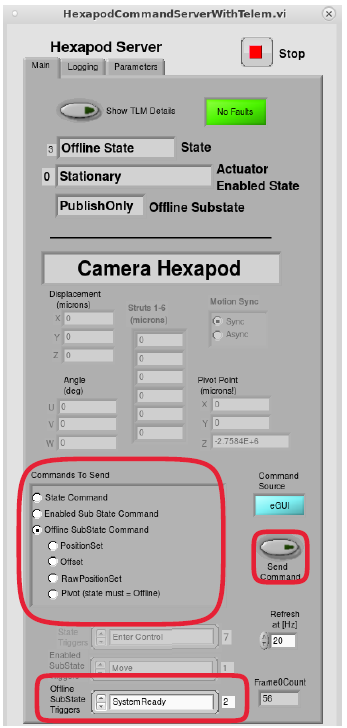
\includegraphics[width=1.79167in]{jira_imgs/1024.png}

}
\hdashrule[0.5ex]{\textwidth}{1pt}{3mm}
  Expected Result \\
{\footnotesize
The system transitions from the OfflineState/PublishOnly substate to the
OfflineState/AvailableState substate and the Command Source says
eGUI.\\[2\baselineskip]

}
\hdashrule[0.5ex]{\textwidth}{1pt}{3mm}
  Actual Result \\
{\footnotesize
We transited the system to the OfflineState/AvailableState substate.

}
\begin{tabular}{p{2cm}p{14cm}}
\toprule
Step 4 & Step Execution Status: \textbf{ Initial Pass } \\ \hline
\end{tabular}
 Description \\
{\footnotesize
\textbf{OFFLINESTATE -\textgreater{} STANDBYSTATE}\\
Click on the State Command field in the Commands to Send section.\\
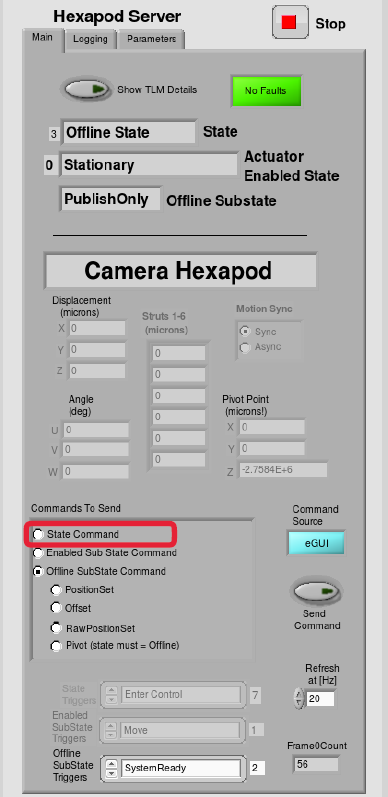
\includegraphics[width=1.79167in]{jira_imgs/1028.png}

}
\hdashrule[0.5ex]{\textwidth}{1pt}{3mm}
  Expected Result \\
{\footnotesize
The State Triggers dialogue box shown below becomes visible.\\
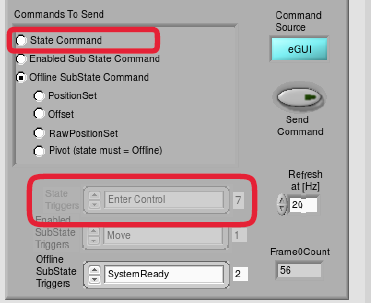
\includegraphics[width=1.79167in]{jira_imgs/1029.png}

}
\hdashrule[0.5ex]{\textwidth}{1pt}{3mm}
  Actual Result \\
{\footnotesize
We transited the system to the Standby state.

}
\begin{tabular}{p{2cm}p{14cm}}
\toprule
Step 5 & Step Execution Status: \textbf{ Initial Pass } \\ \hline
\end{tabular}
 Description \\
{\footnotesize
Scroll through the available trigger options to select ``Enter Control''
and click the Send Command button.

}
\hdashrule[0.5ex]{\textwidth}{1pt}{3mm}
  Expected Result \\
{\footnotesize
The system transitions to the Standby state and the primary state
display box at the top of the Main says Standby State.

}
\hdashrule[0.5ex]{\textwidth}{1pt}{3mm}
  Actual Result \\
{\footnotesize
We transited the system to the Standby state.

}
\begin{tabular}{p{2cm}p{14cm}}
\toprule
Step 6 & Step Execution Status: \textbf{ Initial Pass } \\ \hline
\end{tabular}
 Description \\
{\footnotesize
\textbf{STANDBYSTATE -\textgreater{} DISABLEDSTATE}\\
From the StandbyState, send a Start State command.

}
\hdashrule[0.5ex]{\textwidth}{1pt}{3mm}
  Expected Result \\
{\footnotesize
The system transitions into DisabledState and the current configuration
parameters are maintained from the default parameters or from the
previous DDS start command.~

}
\hdashrule[0.5ex]{\textwidth}{1pt}{3mm}
  Actual Result \\
{\footnotesize
We transited the system to the Disabled state.

}
\begin{tabular}{p{2cm}p{14cm}}
\toprule
Step 7 & Step Execution Status: \textbf{ Initial Pass } \\ \hline
\end{tabular}
 Description \\
{\footnotesize
\textbf{DISABLEDSTATE -\textgreater{} ENABLEDSTATE}\\
From the DisabledState, send an Enable State Command.~

}
\hdashrule[0.5ex]{\textwidth}{1pt}{3mm}
  Expected Result \\
{\footnotesize
The system transitions into the EnabledState/Stationary substate, the
motor drives are enabled and and motion can be commanded.~

}
\hdashrule[0.5ex]{\textwidth}{1pt}{3mm}
  Actual Result \\
{\footnotesize
We transited the system to the Enabled state.

}
\begin{tabular}{p{2cm}p{14cm}}
\toprule
Step 8 & Step Execution Status: \textbf{ Initial Pass } \\ \hline
\end{tabular}
 Description \\
{\footnotesize
\textless{}conditional state\textgreater{}\\
\textbf{FAULTSTATE}\\
If a Fault occurs in any of the other states, the system will
automatically transition to the Fault State. While in the Fault state,
send a clearError.\\
Note: If the fault that occurs goes through the interlock system, reset
the safety relay switch and send a clearError command.

}
\hdashrule[0.5ex]{\textwidth}{1pt}{3mm}
  Expected Result \\
{\footnotesize
The system transitions back to the OfflineState/PublishOnly substate.
(Go back to Step 3)

}
\hdashrule[0.5ex]{\textwidth}{1pt}{3mm}
  Actual Result \\
{\footnotesize
For the safety interlock, press the E-stop first, click the switch
button of release interlock 2, release the E-stop, click the switch
button of reset interlock. By doing this, we could put/ release the
safety interlock. No clearError in software side is
needed.\\[2\baselineskip]When we opened the hexapod GUI, there was the
simulink error after hitting the systemReady command and entered the
Fault state. We can use the clearError to leave the Fault state and do
the state transitions.

}
\begin{tabular}{p{2cm}p{14cm}}
\toprule
Step 9 & Step Execution Status: \textbf{ Fail } \\ \hline
\end{tabular}
 Description \\
{\footnotesize
\textbf{Follow \emph{3.3.1 Positioning} of the LSST Hexapods-Rotator
Acceptance Test Procedure, Sheet 23-24.}

}
\hdashrule[0.5ex]{\textwidth}{1pt}{3mm}
  Test Data \\
 {\footnotesize
\textbf{Deviation:~}Test this with no performance payload and at a
single elevation angle of zero degrees.

}
\hdashrule[0.5ex]{\textwidth}{1pt}{3mm}
  Expected Result \\
{\footnotesize
The position of the hexapod is able to be commanded and no software
limits or limit switches are tripped.

}
\hdashrule[0.5ex]{\textwidth}{1pt}{3mm}
  Actual Result \\
{\footnotesize
Measurements for the positioning could not be completed due to a failure
in drive \#3.\\
1) The tilt angle, tilt offset distance and pivot distance are all OK,
but once reached, the X and Zdon't seem to be able to reach position to
within \textasciitilde{}2mm\\
2) Laser tracker seems to contradict MOOG's statement about corners
representing different combinations of the maximum simultaneous range
requirements for X and Z

}
\hdashrule[0.5ex]{\textwidth}{1pt}{3mm}
  Issues found executing this step:  \\
{\footnotesize
\begin{itemize}
\item \href{https://jira.lsstcorp.org/browse/FRACAS-28}{FRACAS-28}~~Camera Hexapod Drive \#3 Failure

\end{itemize}
}
\begin{tabular}{p{2cm}p{14cm}}
\toprule
Step 10 & Step Execution Status: \textbf{ Initial Pass } \\ \hline
\end{tabular}
 Description \\
{\footnotesize
\textbf{Follow \emph{3.3.2 Centers of Rotation} of the LSST
Hexapods-Rotator Acceptance Test Procedure, Sheet 24-25.}

}
\hdashrule[0.5ex]{\textwidth}{1pt}{3mm}
  Test Data \\
 {\footnotesize
\textbf{Deviation:~}Record pivot position through the EUI.

}
\hdashrule[0.5ex]{\textwidth}{1pt}{3mm}
  Expected Result \\
{\footnotesize
The center of rotation is able to be moved.

}
\hdashrule[0.5ex]{\textwidth}{1pt}{3mm}
  Actual Result \\
{\footnotesize
\emph{COR at 1.938m from the rotator to camera interface}\\
Laser tracker-determined COR: 1930+/-8.2{[}mm{]}\\
\emph{COR at the rotator to camera interface}\\
Laser tracker-determined COR: set value COR 33.75{[}mm{]}; SA measured =
923+/-1 {[}mm{]}\\
Complies with requirement with caveat that there is an offset at the
rotatorsurface: 820.4mm

}
\begin{tabular}{p{2cm}p{14cm}}
\toprule
Step 11 & Step Execution Status: \textbf{ Initial Pass } \\ \hline
\end{tabular}
 Description \\
{\footnotesize
\textbf{Follow \emph{3.3.3 Cross-Talk Motion~}of the LSST
Hexapods-Rotator Acceptance Test Procedure, Sheet 25.}

}
\hdashrule[0.5ex]{\textwidth}{1pt}{3mm}
  Expected Result \\
{\footnotesize
There is no cross-talk observed (actuator positioning errors and
erroneous geometry are minimal)

}
\hdashrule[0.5ex]{\textwidth}{1pt}{3mm}
  Actual Result \\
{\footnotesize
Based on rest of tests

}
\begin{tabular}{p{2cm}p{14cm}}
\toprule
Step 12 & Step Execution Status: \textbf{ Initial Pass } \\ \hline
\end{tabular}
 Description \\
{\footnotesize
\textbf{Follow \emph{3.3.4 Radial (X and Y) Translational Range~}of the
LSST Hexapods-Rotator Acceptance Test Procedure, Sheet 25.}

}
\hdashrule[0.5ex]{\textwidth}{1pt}{3mm}
  Test Data \\
 {\footnotesize
\textbf{Deviation:~}Only test at a zero degree elevation angle.

}
\hdashrule[0.5ex]{\textwidth}{1pt}{3mm}
  Expected Result \\
{\footnotesize
The hexapod is capable of moving to the positions in the XY plane listed
in the Acceptance Test Procedure.

}
\hdashrule[0.5ex]{\textwidth}{1pt}{3mm}
  Actual Result \\
{\footnotesize
1. 7.57428275,0,0,0,0,0\\
2. 5.3578403, 5.37473926,0,0,0,0\\
3. 0,7.58852237,0,0,0,0\\
4. -5.34249993, 5.33297113,0,0,0,0\\
5. -7.57839578,0,0,0,0,0\\
6. -5.34249993, -5.38597352,0,0,0,0\\
7. 0;-7.55189491,0,0,0,0\\
8. 5.3578403; -5.34205358;0;0;0;0

}
\begin{tabular}{p{2cm}p{14cm}}
\toprule
Step 13 & Step Execution Status: \textbf{ Initial Pass } \\ \hline
\end{tabular}
 Description \\
{\footnotesize
\textbf{Follow \emph{3.3.6 Axial (Z) Translation Range~}of the LSST
Hexapods-Rotator Acceptance Test Procedure, Sheet 27.}

}
\hdashrule[0.5ex]{\textwidth}{1pt}{3mm}
  Test Data \\
 {\footnotesize
\textbf{Deviation:~}Only test at a zero degree elevation angle.

}
\hdashrule[0.5ex]{\textwidth}{1pt}{3mm}
  Expected Result \\
{\footnotesize
The hexapod is capable of moving to the positions in the Z plane listed
in the Acceptance Test Procedure.~

}
\hdashrule[0.5ex]{\textwidth}{1pt}{3mm}
  Actual Result \\
{\footnotesize
1. 0;0;8.72487391;0;0;0\\
2. 0,0, -8.710510168,0,0,0\\
3. 0;0;8.70619302;0;0;0

}
\begin{tabular}{p{2cm}p{14cm}}
\toprule
Step 14 & Step Execution Status: \textbf{ Initial Pass } \\ \hline
\end{tabular}
 Description \\
{\footnotesize
\textbf{Follow \emph{3.3.8 Rotational Range Around X-Axis (Tip) and
Y-Axis (Tilt)~}of the LSST Hexapods-Rotator Acceptance Test Procedure,
Sheet 28-29.}

}
\hdashrule[0.5ex]{\textwidth}{1pt}{3mm}
  Test Data \\
 {\footnotesize
\textbf{Deviation:~}Only test at a zero degree elevation angle.

}
\hdashrule[0.5ex]{\textwidth}{1pt}{3mm}
  Expected Result \\
{\footnotesize
The hexapod is capable of moving to the positions in the RXRY plane
listed in the Acceptance Test Procedure.

}
\hdashrule[0.5ex]{\textwidth}{1pt}{3mm}
  Actual Result \\
{\footnotesize
Command (0,0,0,0.24 deg,0,0): (0,0,0,0.2429,0,0)\\
Command (0,0,0,0.170deg,0.170deg,0): (0,0,0,0.1732,0.1707,0)\\
Command (0,0,0,0,0.24deg,0): (0,0,0,0.2402,0,0)\\
Command (0,0,0,-0.170deg,0.170deg,0): (0,0,0,-0.1689,0.1714,0)\\
Command (0,0,0,-0.24deg,0,0): (0,0,0,-0.2414,0,0)\\
Command (0,0,0,-0.170deg,-0.170deg,0): (0,0,0,-0.169,-0.1703,0)\\
Command (0,0,0,0,-0.24deg,0): (0,0,0,0,-0.2431,0)\\
Command (0,0,0,0.170deg,-0.170deg,0):
(0,0,0,0.173,-0.1714,0)\\[2\baselineskip]Measurements error
STDEV\textless{}0.00205Deg

}
\begin{tabular}{p{2cm}p{14cm}}
\toprule
Step 15 & Step Execution Status: \textbf{ Initial Pass } \\ \hline
\end{tabular}
 Description \\
{\footnotesize
\textbf{Follow \emph{3.3.10 Rotation Range Around Z-Axis (Twist)~}of the
LSST Hexapods-Rotator Acceptance Test Procedure, Sheet 30.}

}
\hdashrule[0.5ex]{\textwidth}{1pt}{3mm}
  Test Data \\
 {\footnotesize
\textbf{Deviation:~}Only test at a zero degree elevation angle.

}
\hdashrule[0.5ex]{\textwidth}{1pt}{3mm}
  Expected Result \\
{\footnotesize
The hexapod is capable of moving to the positions in the RZ-axis listed
in the Acceptance Test Procedure.

}
\hdashrule[0.5ex]{\textwidth}{1pt}{3mm}
  Actual Result \\
{\footnotesize
Command (0,0,0,0,0,0.1deg): (0,0,0,0,0,0.0999)\\
Command (0,0,0,0,0,-0.1deg): (0,0,0,0,0,-0.09955)\\[2\baselineskip]Error
\textless{} 0.015Deg

}
\begin{tabular}{p{2cm}p{14cm}}
\toprule
Step 16 & Step Execution Status: \textbf{ Not Executed } \\ \hline
\end{tabular}
 Description \\
{\footnotesize
\textbf{Follow \emph{3.3.12 Hexapod Repeatability} of the LSST
Hexapods-Rotato Acceptance Test Procedure, Sheet 31.}

}
\hdashrule[0.5ex]{\textwidth}{1pt}{3mm}
  Expected Result \\
{\footnotesize
The repeatability is as good as the test equipment can capture. This
means that the repeatability is limited by the resolution of the test
equipment.

}
\hdashrule[0.5ex]{\textwidth}{1pt}{3mm}
  Actual Result \\
{\footnotesize

}
\begin{tabular}{p{2cm}p{14cm}}
\toprule
Step 17 & Step Execution Status: \textbf{ Initial Pass } \\ \hline
\end{tabular}
 Description \\
{\footnotesize
\textbf{Follow \emph{3.3.13 Hexapod Absolute Accuracy~}of the LSST
Hexapods-Rotator Acceptance Test Procedure, Sheet 38-42.}

}
\hdashrule[0.5ex]{\textwidth}{1pt}{3mm}
  Test Data \\
 {\footnotesize
\textbf{Deviation:~}Only test at a zero degree elevation angle.

}
\hdashrule[0.5ex]{\textwidth}{1pt}{3mm}
  Expected Result \\
{\footnotesize
The accuracy of the hexapod is good enough to be consistently repeated.

}
\hdashrule[0.5ex]{\textwidth}{1pt}{3mm}
  Actual Result \\
{\footnotesize
Shall be done in test cases 12-15.

}
\begin{tabular}{p{2cm}p{14cm}}
\toprule
Step 18 & Step Execution Status: \textbf{ Initial Pass } \\ \hline
\end{tabular}
 Description \\
{\footnotesize
\textbf{Follow \emph{3.3.16 Hexapod Radial (X and Y) and Axial (Z)
Velocity Range} and~\emph{3.3.17 Hexapod Rotational Velocity~}of the
LSST Hexapods-Rotator Acceptance Test Procedure, Sheet 43-44.}

}
\hdashrule[0.5ex]{\textwidth}{1pt}{3mm}
  Test Data \\
 {\footnotesize
\textbf{Deviation:~}Only test this using synchronous mode.

}
\hdashrule[0.5ex]{\textwidth}{1pt}{3mm}
  Expected Result \\
{\footnotesize
The hexapod velocity exceeds the 152um/s in XY and 0.0039deg/s in RXYRY
and RZ requirements.

}
\hdashrule[0.5ex]{\textwidth}{1pt}{3mm}
  Actual Result \\
{\footnotesize
Hexapod meets requirements.

}
\begin{tabular}{p{2cm}p{14cm}}
\toprule
Step 19 & Step Execution Status: \textbf{ Not Executed } \\ \hline
\end{tabular}
 Description \\
{\footnotesize
\textbf{Follow \emph{3.3.18 Hexapod Heat Dissipation~}of the LSST
Hexapods-Rotator Acceptance Test Procedure, Sheet 44.}

}
\hdashrule[0.5ex]{\textwidth}{1pt}{3mm}
  Expected Result \\
{\footnotesize
The current measured by the inductive current probes is calculated to
meet the heat dissipation requirement.

}
\hdashrule[0.5ex]{\textwidth}{1pt}{3mm}
  Actual Result \\
{\footnotesize
As this was originally tested with a surrogate mass, this step was left
unexecuted and will be tested in the future with ComCam (with load).~

}

\paragraph{ LVV-T1599 - Camera Hexapod Software Functional Re-verification }\mbox{}\\

Version \textbf{1}.
Open  \href{https://jira.lsstcorp.org/secure/Tests.jspa#/testCase/LVV-T1599}{\textit{ LVV-T1599 } }
test case in Jira.

The objective of this test case is to re-verify the functional
requirements of the camera hexapod's software, after shipment of the
hardware from the vendor's facility to the Summit, as defined in \citeds{LTS-206}
and \citeds{LTS-160}. This test case will only exercise the functionality that
was executed previously and meets the following criteria:

\begin{itemize}
\tightlist
\item
  Only requires the camera hexapod to be operable
\item
  Only requires testing of the synchronous mode

  \begin{itemize}
  \tightlist
  \item
    \textbf{Asynchronous mode is not a standard mode of operation}
  \end{itemize}
\item
  Only requires the vendors EUI software and hardware via local control

  \begin{itemize}
  \tightlist
  \item
    Does \textbf{NOT} require integration with SAL
  \end{itemize}
\item
  Does \textbf{NOT} require the camera hexapod to be loaded with the
  camera simulated mass or actual camera hardware
\end{itemize}

The software functional requirements were previously verified during the
test campaign by the vendor at the vendor's facility and accepted by
LSST during the Factory Acceptance Test review. The test procedure used
during the vendor's acceptance testing is the \emph{LSST
Hexapods-Rotator Software Acceptance Test Procedure} which is attached
to this test case. The test steps of this test case are taken directly
from that document on how to perform the test in a similar way as was
performed previously and includes changes noted by the
vendor.\\[2\baselineskip]See the attached \emph{LSST Hexapod Operator's
Manual} for more information on how to operate the hexapod.

\textbf{ Preconditions}:\\
Prior to the execution of this test case to re-verify the Camera Hexapod
hardware functional requirements, the following Summit tasks must be
completed:

\begin{itemize}
\tightlist
\item
  The Hexapod has been installed on the camera cart

  \begin{itemize}
  \tightlist
  \item
    \url{https://jira.lsstcorp.org/browse/SUMMIT-3224}
  \end{itemize}
\item
  The Hexapod Controller has been deployed on the summit

  \begin{itemize}
  \tightlist
  \item
    \url{https://jira.lsstcorp.org/browse/SUMMIT-3229}
  \end{itemize}
\item
  Boxes for the Hexapod have been transported to the 3rd level

  \begin{itemize}
  \tightlist
  \item
    \url{https://jira.lsstcorp.org/browse/SUMMIT-3230}
  \end{itemize}
\item
  All Hexapod cables and cabinets have been prepared for integration
  with camera cart

  \begin{itemize}
  \tightlist
  \item
    \url{https://jira.lsstcorp.org/browse/SUMMIT-3231}
  \end{itemize}
\item
  The offset has been installed onto the integrating structure

  \begin{itemize}
  \tightlist
  \item
    \url{https://jira.lsstcorp.org/browse/SUMMIT-3293}
  \end{itemize}
\item
  The Camera Hexapod electrical connections have been tested

  \begin{itemize}
  \tightlist
  \item
    \url{https://jira.lsstcorp.org/browse/SUMMIT-3294}
  \end{itemize}
\end{itemize}

Execution status: {\bf Initial Pass }

Final comment:\\


Detailed steps results:

\begin{tabular}{p{2cm}p{14cm}}
\toprule
Step 1 & Step Execution Status: \textbf{ Initial Pass } \\ \hline
\end{tabular}
 Description \\
{\footnotesize
\textbf{STARTING THE EUI}\\[2\baselineskip]Double click the Hexapod GUI
Viewer desktop icon on the computer.

\begin{itemize}
\tightlist
\item
  This can be done on the Dell Management PC or another computer on the
  same network
\end{itemize}

}
\hdashrule[0.5ex]{\textwidth}{1pt}{3mm}
  Expected Result \\
{\footnotesize
A prompt to enter the password is shown.

}
\hdashrule[0.5ex]{\textwidth}{1pt}{3mm}
  Actual Result \\
{\footnotesize
We saw the prompt window and asked for the password.

}
\begin{tabular}{p{2cm}p{14cm}}
\toprule
Step 2 & Step Execution Status: \textbf{ Initial Pass } \\ \hline
\end{tabular}
 Description \\
{\footnotesize
Enter the password ``lsst-vnc''

\begin{itemize}
\tightlist
\item
  If the EUI isn't automatically up and running when the VNC opens,
  double click on the Hexapod-eGUI icon on the VNC viewer
\end{itemize}

}
\hdashrule[0.5ex]{\textwidth}{1pt}{3mm}
  Expected Result \\
{\footnotesize
The EUI is in the Offline State/PublishOnly substate and is able to
publish through SAL but cannot receive commands.

}
\hdashrule[0.5ex]{\textwidth}{1pt}{3mm}
  Actual Result \\
{\footnotesize
After we entered the ``lsst-vnc'', we can log in the system. The initial
state is Offline State/PublishOnly. We saw the green light of DDS
connected.

}
\begin{tabular}{p{2cm}p{14cm}}
\toprule
Step 3 & Step Execution Status: \textbf{ Initial Pass } \\ \hline
\end{tabular}
 Description \\
{\footnotesize
\textbf{OFFLINESTATE/AVAILABLESTATE}\\
On the Main tab, select the ``Offline SubState Cmd'' field in the
Commands to Send section, set the Offline SubState Triggers to ``System
Ready'' and click on the Send Command button.\\
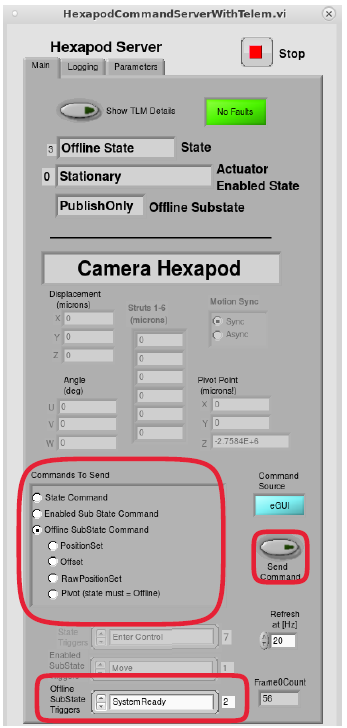
\includegraphics[width=1.79167in]{jira_imgs/1024.png}

}
\hdashrule[0.5ex]{\textwidth}{1pt}{3mm}
  Expected Result \\
{\footnotesize
The system transitions from the OfflineState/PublishOnly substate to the
OfflineState/AvailableState substate and the Command Source says
eGUI.\\[2\baselineskip]

}
\hdashrule[0.5ex]{\textwidth}{1pt}{3mm}
  Actual Result \\
{\footnotesize
We transited the system to the OfflineState/AvailableState substate.

}
\begin{tabular}{p{2cm}p{14cm}}
\toprule
Step 4 & Step Execution Status: \textbf{ Initial Pass } \\ \hline
\end{tabular}
 Description \\
{\footnotesize
\textbf{OFFLINESTATE -\textgreater{} STANDBYSTATE}\\
Click on the State Command field in the Commands to Send section.\\
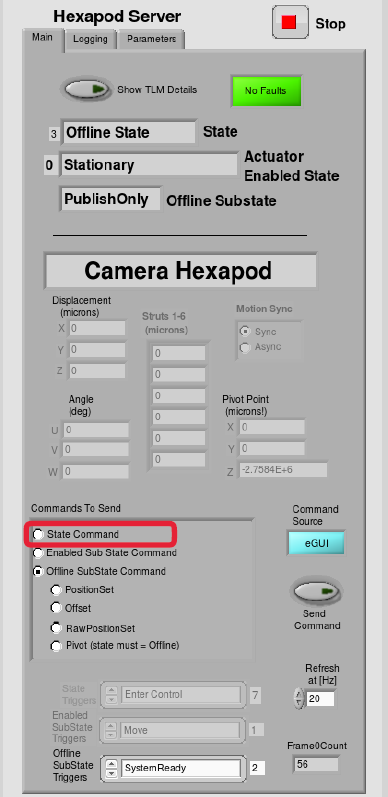
\includegraphics[width=1.79167in]{jira_imgs/1028.png}

}
\hdashrule[0.5ex]{\textwidth}{1pt}{3mm}
  Expected Result \\
{\footnotesize
The State Triggers dialogue box shown below becomes visible.\\
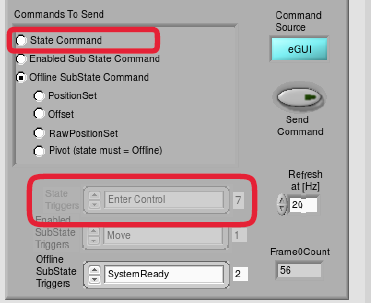
\includegraphics[width=1.79167in]{jira_imgs/1029.png}

}
\hdashrule[0.5ex]{\textwidth}{1pt}{3mm}
  Actual Result \\
{\footnotesize
We transited the system to the Standby state.

}
\begin{tabular}{p{2cm}p{14cm}}
\toprule
Step 5 & Step Execution Status: \textbf{ Initial Pass } \\ \hline
\end{tabular}
 Description \\
{\footnotesize
Scroll through the available trigger options to select ``Enter Control''
and click the Send Command button.

}
\hdashrule[0.5ex]{\textwidth}{1pt}{3mm}
  Expected Result \\
{\footnotesize
The system transitions to the Standby state and the primary state
display box at the top of the Main says Standby State.

}
\hdashrule[0.5ex]{\textwidth}{1pt}{3mm}
  Actual Result \\
{\footnotesize
We transited the system to the Standby state.

}
\begin{tabular}{p{2cm}p{14cm}}
\toprule
Step 6 & Step Execution Status: \textbf{ Initial Pass } \\ \hline
\end{tabular}
 Description \\
{\footnotesize
\textbf{STANDBYSTATE -\textgreater{} DISABLEDSTATE}\\
From the StandbyState, send a Start State command.

}
\hdashrule[0.5ex]{\textwidth}{1pt}{3mm}
  Expected Result \\
{\footnotesize
The system transitions into DisabledState and the current configuration
parameters are maintained from the default parameters or from the
previous DDS start command.~

}
\hdashrule[0.5ex]{\textwidth}{1pt}{3mm}
  Actual Result \\
{\footnotesize
Duplication of the test case 6 in LVV-T1598.

}
\begin{tabular}{p{2cm}p{14cm}}
\toprule
Step 7 & Step Execution Status: \textbf{ Initial Pass } \\ \hline
\end{tabular}
 Description \\
{\footnotesize
\textbf{DISABLEDSTATE -\textgreater{} ENABLEDSTATE}\\
From the DisabledState, send an Enable State Command.~

}
\hdashrule[0.5ex]{\textwidth}{1pt}{3mm}
  Expected Result \\
{\footnotesize
The system transitions into the EnabledState/Stationary substate, the
motor drives are enabled and and motion can be commanded.~

}
\hdashrule[0.5ex]{\textwidth}{1pt}{3mm}
  Actual Result \\
{\footnotesize
We transited the system to the Disabled state.

}
\begin{tabular}{p{2cm}p{14cm}}
\toprule
Step 8 & Step Execution Status: \textbf{ Initial Pass } \\ \hline
\end{tabular}
 Description \\
{\footnotesize
\textless{}conditional state\textgreater{}\\
\textbf{FAULTSTATE}\\
If a Fault occurs in any of the other states, the system will
automatically transition to the Fault State. While in the Fault state,
send a clearError.\\
Note: If the fault that occurs goes through the interlock system, reset
the safety relay switch and send a clearError command.

}
\hdashrule[0.5ex]{\textwidth}{1pt}{3mm}
  Expected Result \\
{\footnotesize
The system transitions back to the OfflineState/PublishOnly substate.
(Go back to Step 3)

}
\hdashrule[0.5ex]{\textwidth}{1pt}{3mm}
  Actual Result \\
{\footnotesize
For the safety interlock, press the E-top first, click the switch button
of release interlock 2, release the E-stop, click the switch button of
reset interlock. By doing this, we could put/ release the safety
interlock. No clearError in software side is
needed.\\[2\baselineskip]When we opened the hexapod GUI, there was the
simulink error after hitting the systemReady command and entered the
Fault state. We can use the clearError to leave the Fault state and do
the state transitions.

}
\begin{tabular}{p{2cm}p{14cm}}
\toprule
Step 9 & Step Execution Status: \textbf{ Initial Pass } \\ \hline
\end{tabular}
 Description \\
{\footnotesize
\textbf{Section 3.1.1 of the attached Software Acceptance Test
Procedure\\
Test Sequence \#1 - Synchronous PositionSet and Move
Commands}\\[2\baselineskip]With the synchronous button enabled and in
enabled/stationary state, send a positionSet command of (0um, 0um,
200um, 0 deg, 0 deg, 0 deg) using the EUI.

}
\hdashrule[0.5ex]{\textwidth}{1pt}{3mm}
  Expected Result \\
{\footnotesize
The hexapod doesn't move.

}
\hdashrule[0.5ex]{\textwidth}{1pt}{3mm}
  Actual Result \\
{\footnotesize
We sent the positionSet command of (0um, 0um, 200um, 0 deg, 0 deg, 0
deg) only and the hexapod did not move.

}
\begin{tabular}{p{2cm}p{14cm}}
\toprule
Step 10 & Step Execution Status: \textbf{ Initial Pass } \\ \hline
\end{tabular}
 Description \\
{\footnotesize
With the synchronous button enabled and in enabled/stationary state,
send a positionSet command of (2000um, -3500um, 200um, .01 deg, -.05deg,
.002deg) using the EUI.

}
\hdashrule[0.5ex]{\textwidth}{1pt}{3mm}
  Expected Result \\
{\footnotesize
The hexapod doesn't move.

}
\hdashrule[0.5ex]{\textwidth}{1pt}{3mm}
  Actual Result \\
{\footnotesize
We sent the positionSet command of (2000um, -3500um, 200um, .01 deg,
-.05deg, .002deg) only and the hexapod did not move.

}
\begin{tabular}{p{2cm}p{14cm}}
\toprule
Step 11 & Step Execution Status: \textbf{ Initial Pass } \\ \hline
\end{tabular}
 Description \\
{\footnotesize
Send a move command using the EUI.

}
\hdashrule[0.5ex]{\textwidth}{1pt}{3mm}
  Expected Result \\
{\footnotesize
The hexapod moves to the last commanded position of (2000um, -3500um,
200um, .01 deg, -.05deg, .002deg) and the actuators complete the move at
nearly the same time as seen on the motion complete lights on the
telemetry screen.

}
\hdashrule[0.5ex]{\textwidth}{1pt}{3mm}
  Actual Result \\
{\footnotesize
We saw the movement of hexapod with position (2000um, -3500um, 200um,
.01 deg, -.05deg, .002deg) after hitting the move command. The final
position is (1999um, -3500um, 200um, .01 deg, -.05deg, .002deg) on GUI.
We saw a ``1 um'' difference in x position.

}
\begin{tabular}{p{2cm}p{14cm}}
\toprule
Step 12 & Step Execution Status: \textbf{ Initial Pass } \\ \hline
\end{tabular}
 Description \\
{\footnotesize
\textbf{Section 3.1.1 of the attached Software Acceptance Test
Procedure\\
Test Sequence \#2 - Pivot, PositionSet and Move
Commands}\\[2\baselineskip]In enabled/stationary state and at the last
commanded position of (2000um, -3500um, 200um, .01 deg, -.05deg,
.002deg), change the pivot point from the default location to (0,0,0)
using the EUI.

}
\hdashrule[0.5ex]{\textwidth}{1pt}{3mm}
  Expected Result \\
{\footnotesize
The actuator positions do not change, but the hexapod position is
(-407um, -3982um, 199um, 0.01deg, -0.05deg, 0.002deg)

}
\hdashrule[0.5ex]{\textwidth}{1pt}{3mm}
  Actual Result \\
{\footnotesize
The default pivot position is (0, 0, -2758400um). Change the pivot to
(0, 0, 0) in the offline state (it can not be changed in the enabled
state). The hexapod position is (-408um, -3982um, 199um, 0.01deg,
-0.05deg, 0.002deg). The x position differs by 1 um from the case
11.\\[2\baselineskip]PS. The pivot value can only be changed in the
offline state not enabled/stationary state. There will be a prompt
window to complain the wrong state.

}
\begin{tabular}{p{2cm}p{14cm}}
\toprule
Step 13 & Step Execution Status: \textbf{ Initial Pass } \\ \hline
\end{tabular}
 Description \\
{\footnotesize
In the enabled/stationary state, send a positionSet command of (2000um,
-3500um, 200um, .01 deg, -.05deg, .002deg) using the EUI.

}
\hdashrule[0.5ex]{\textwidth}{1pt}{3mm}
  Expected Result \\
{\footnotesize
The hexapod doesn't move.

}
\hdashrule[0.5ex]{\textwidth}{1pt}{3mm}
  Actual Result \\
{\footnotesize
We sent the positionSet command of (2000um, -3500um, 200um, .01 deg,
-.05deg, .002deg) only and the hexapod did not move.

}
\begin{tabular}{p{2cm}p{14cm}}
\toprule
Step 14 & Step Execution Status: \textbf{ Initial Pass } \\ \hline
\end{tabular}
 Description \\
{\footnotesize
Send a move command using the EUI.

}
\hdashrule[0.5ex]{\textwidth}{1pt}{3mm}
  Expected Result \\
{\footnotesize
The hexapod moves to the commanded position of (2000um, -3500um, 200um,
.01 deg, -.05deg, .002deg) and the actuators change position to account
for the new pivot point.

}
\hdashrule[0.5ex]{\textwidth}{1pt}{3mm}
  Actual Result \\
{\footnotesize
The hexapod moved to the position of (2000um, -3500um, 200um, .01 deg,
-.05deg, .002deg) based on GUI with the new pivot point.

}
\begin{tabular}{p{2cm}p{14cm}}
\toprule
Step 15 & Step Execution Status: \textbf{ Initial Pass } \\ \hline
\end{tabular}
 Description \\
{\footnotesize
\textbf{Section 3.1.1 of the attached Software Acceptance Test
Procedure\\
Test Sequence \#4 - Synchronous Offset and Move
Commands}\\[2\baselineskip]With the synchronous button enabled and in
enabled/stationary state, send a positionSet command of (500um, 800um,
200um, 0 deg, 0 deg, 0 deg).

}
\hdashrule[0.5ex]{\textwidth}{1pt}{3mm}
  Expected Result \\
{\footnotesize
The hexapod doesn't move.

}
\hdashrule[0.5ex]{\textwidth}{1pt}{3mm}
  Actual Result \\
{\footnotesize
We sent the positionSet command of (500um, 800um, 200um, 0 deg, 0 deg, 0
deg) only and the hexapod did not move.

}
\begin{tabular}{p{2cm}p{14cm}}
\toprule
Step 16 & Step Execution Status: \textbf{ Initial Pass } \\ \hline
\end{tabular}
 Description \\
{\footnotesize
With the synchronous button enabled and in enabled/stationary state,
send an offset command of (0um, 0um, 2000um, 0 deg, 0 deg, 0 deg).~

}
\hdashrule[0.5ex]{\textwidth}{1pt}{3mm}
  Expected Result \\
{\footnotesize
The hexapod doesn't move.

}
\hdashrule[0.5ex]{\textwidth}{1pt}{3mm}
  Actual Result \\
{\footnotesize
We sent the offset command of (0um, 0um, 2000um, 0 deg, 0 deg, 0 deg)
only and the hexapod did not move.

}
\begin{tabular}{p{2cm}p{14cm}}
\toprule
Step 17 & Step Execution Status: \textbf{ Initial Pass } \\ \hline
\end{tabular}
 Description \\
{\footnotesize
Send a move command.

}
\hdashrule[0.5ex]{\textwidth}{1pt}{3mm}
  Expected Result \\
{\footnotesize
The hexapod moves only 2000um in Z from the previous position and the
actuators complete the move at nearly the same time as seen on the
motion complete lights on the telemetry screen.

}
\hdashrule[0.5ex]{\textwidth}{1pt}{3mm}
  Actual Result \\
{\footnotesize
Put the hexapod to origin. Do the case 15 and 16 and move. The hexapod
moves to (1um, 0, 2000um, 0, 0, 0). We saw the offset command will
override the positionSet command from case 15.

}
\begin{tabular}{p{2cm}p{14cm}}
\toprule
Step 18 & Step Execution Status: \textbf{ Initial Pass } \\ \hline
\end{tabular}
 Description \\
{\footnotesize
\textbf{Instead of Asynchronous Test}\\
{With the synchronous button enabled and in enabled/stationary
state,}{\textbf{~}}{s}end a position set command of (0um, 0um, 0um,
0.1deg, 0deg, 0deg)

}
\hdashrule[0.5ex]{\textwidth}{1pt}{3mm}
  Expected Result \\
{\footnotesize
The hexapod doesn't move.

}
\hdashrule[0.5ex]{\textwidth}{1pt}{3mm}
  Actual Result \\
{\footnotesize
We sent the positionSet command of (0, 0, 0, 0.1deg, 0, 0) only and the
hexapod did not move.

}
\begin{tabular}{p{2cm}p{14cm}}
\toprule
Step 19 & Step Execution Status: \textbf{ Initial Pass } \\ \hline
\end{tabular}
 Description \\
{\footnotesize
Send a move command.

}
\hdashrule[0.5ex]{\textwidth}{1pt}{3mm}
  Expected Result \\
{\footnotesize
The hexapod moves to the commanded position of (0um, 0um, 0um, 0.1deg,
0deg, 0deg)

}
\hdashrule[0.5ex]{\textwidth}{1pt}{3mm}
  Actual Result \\
{\footnotesize
1. The hexapod moved to (0 , -2um, 0, 0.1deg, 0, 0) based on GUI from
the (1um, 0, 2000um, 0, 0, 0) in case 17.\\
2. The hexapod moved to (0 , 1um, 0, 0.1deg, 0, 0) based on GUI from the
origin (0, -1um, 0, 0, 0, 0).

}
\begin{tabular}{p{2cm}p{14cm}}
\toprule
Step 20 & Step Execution Status: \textbf{ Initial Pass } \\ \hline
\end{tabular}
 Description \\
{\footnotesize
With the synchronous button enabled and in enabled/stationary
state,\textbf{~}send a position set command of (0um, 0um, 0um, 0deg,
0.1deg, 0deg)

}
\hdashrule[0.5ex]{\textwidth}{1pt}{3mm}
  Expected Result \\
{\footnotesize
The hexapod doesn't move.

}
\hdashrule[0.5ex]{\textwidth}{1pt}{3mm}
  Actual Result \\
{\footnotesize
We sent the positionSet command of (0, 0, 0, 0, 0.1deg, 0) only and the
hexapod did not move.

}
\begin{tabular}{p{2cm}p{14cm}}
\toprule
Step 21 & Step Execution Status: \textbf{ Initial Pass } \\ \hline
\end{tabular}
 Description \\
{\footnotesize
Send a move command.

}
\hdashrule[0.5ex]{\textwidth}{1pt}{3mm}
  Expected Result \\
{\footnotesize
The hexapod moves to the commanded position of (0um, 0um, 0um, 0deg,
0.1deg, 0deg)

}
\hdashrule[0.5ex]{\textwidth}{1pt}{3mm}
  Actual Result \\
{\footnotesize
The hexapod moved to (0 , -1um, 0, 0, 0.1deg, 0) based on GUI from the
origin (0, -1um, 0, 0, 0, 0).

}
\begin{tabular}{p{2cm}p{14cm}}
\toprule
Step 22 & Step Execution Status: \textbf{ Initial Pass } \\ \hline
\end{tabular}
 Description \\
{\footnotesize
With the synchronous button enabled and in enabled/stationary
state,\textbf{~}send a position set command of (0um, 0um, 0um, 0.1deg,
0.1deg, 0deg)

}
\hdashrule[0.5ex]{\textwidth}{1pt}{3mm}
  Expected Result \\
{\footnotesize
The hexapod doesn't move.

}
\hdashrule[0.5ex]{\textwidth}{1pt}{3mm}
  Actual Result \\
{\footnotesize
We sent the positionSet command of (0, 0, 0, 0.1deg, 0.1deg, 0) only and
the hexapod did not move.

}
\begin{tabular}{p{2cm}p{14cm}}
\toprule
Step 23 & Step Execution Status: \textbf{ Initial Pass } \\ \hline
\end{tabular}
 Description \\
{\footnotesize
Send a move command.

}
\hdashrule[0.5ex]{\textwidth}{1pt}{3mm}
  Expected Result \\
{\footnotesize
The hexapod moves to the commanded position of (0um, 0um, 0um, 0.1deg,
0.1deg, 0deg)

}
\hdashrule[0.5ex]{\textwidth}{1pt}{3mm}
  Actual Result \\
{\footnotesize
The hexapod moved to (0 , 0, 0, 0.1deg, 0.1deg, 0) based on GUI from the
origin (0, 0, 0, 0, 0, 0).

}
\begin{tabular}{p{2cm}p{14cm}}
\toprule
Step 24 & Step Execution Status: \textbf{ Initial Pass } \\ \hline
\end{tabular}
 Description \\
{\footnotesize
\textbf{Section 3.1.1 of the attached Software Acceptance Test
Procedure\\
Test Sequence \#5 - Stop Commands}\\[2\baselineskip]In
enabled/stationary state, send a position set command of (0um, 0um,
5000um, 0 deg, 0 deg, 0 deg).

}
\hdashrule[0.5ex]{\textwidth}{1pt}{3mm}
  Expected Result \\
{\footnotesize
The hexapod doesn't move.

}
\hdashrule[0.5ex]{\textwidth}{1pt}{3mm}
  Actual Result \\
{\footnotesize
We sent the positionSet command of (0, 0, 5000um, 0, 0, 0) only and the
hexapod did not move.

}
\begin{tabular}{p{2cm}p{14cm}}
\toprule
Step 25 & Step Execution Status: \textbf{ Initial Pass } \\ \hline
\end{tabular}
 Description \\
{\footnotesize
Send a move command.

}
\hdashrule[0.5ex]{\textwidth}{1pt}{3mm}
  Expected Result \\
{\footnotesize
The hexapod starts to move to the commanded position.

}
\hdashrule[0.5ex]{\textwidth}{1pt}{3mm}
  Actual Result \\
{\footnotesize
The hexapod was moving to to (0 , 0, ~5000um, 0, 0, 0) based on GUI from
the origin (1um, 0, 0, 0, 0, 0).

}
\begin{tabular}{p{2cm}p{14cm}}
\toprule
Step 26 & Step Execution Status: \textbf{ Initial Pass } \\ \hline
\end{tabular}
 Description \\
{\footnotesize
While the hexapod is moving, send a stop command.~

}
\hdashrule[0.5ex]{\textwidth}{1pt}{3mm}
  Expected Result \\
{\footnotesize
The hexapod quickly comes to a stop prior to reaching the commanded
position.

}
\hdashrule[0.5ex]{\textwidth}{1pt}{3mm}
  Actual Result \\
{\footnotesize
The hexapod stopped at the position of (0, 0, 2300um , 0, 0, 0).

}
\begin{tabular}{p{2cm}p{14cm}}
\toprule
Step 27 & Step Execution Status: \textbf{ Initial Pass } \\ \hline
\end{tabular}
 Description \\
{\footnotesize
\textbf{Section 3.3.1 EUI Tests of the attached Software Acceptance Test
Procedure}\\
At startup, confirm that the system starts in the Offline/PublishOnly
state.

}
\hdashrule[0.5ex]{\textwidth}{1pt}{3mm}
  Expected Result \\
{\footnotesize
The rotator starts in the Offline/PublishOnly state.

}
\hdashrule[0.5ex]{\textwidth}{1pt}{3mm}
  Actual Result \\
{\footnotesize
It is the Offline/PublishOnly state at startup.

}
\begin{tabular}{p{2cm}p{14cm}}
\toprule
Step 28 & Step Execution Status: \textbf{ Initial Pass } \\ \hline
\end{tabular}
 Description \\
{\footnotesize
Send an offline substate trigger of systemReady.

}
\hdashrule[0.5ex]{\textwidth}{1pt}{3mm}
  Expected Result \\
{\footnotesize
The system transitions into the Offline/Available substate.

}
\hdashrule[0.5ex]{\textwidth}{1pt}{3mm}
  Actual Result \\
{\footnotesize
The system transited to Offline/Available substate.

}
\begin{tabular}{p{2cm}p{14cm}}
\toprule
Step 29 & Step Execution Status: \textbf{ Initial Pass } \\ \hline
\end{tabular}
 Description \\
{\footnotesize
Send an EnterControl trigger.

}
\hdashrule[0.5ex]{\textwidth}{1pt}{3mm}
  Expected Result \\
{\footnotesize
The system transitions from Offline/Available to Standby state.

}
\hdashrule[0.5ex]{\textwidth}{1pt}{3mm}
  Actual Result \\
{\footnotesize
The system transited to Standby state.

}
\begin{tabular}{p{2cm}p{14cm}}
\toprule
Step 30 & Step Execution Status: \textbf{ Initial Pass } \\ \hline
\end{tabular}
 Description \\
{\footnotesize
Send a Start trigger.

}
\hdashrule[0.5ex]{\textwidth}{1pt}{3mm}
  Expected Result \\
{\footnotesize
The system transitions from Standby to Disabled state.

}
\hdashrule[0.5ex]{\textwidth}{1pt}{3mm}
  Actual Result \\
{\footnotesize
The system transited to Disabled state.

}
\begin{tabular}{p{2cm}p{14cm}}
\toprule
Step 31 & Step Execution Status: \textbf{ Initial Pass } \\ \hline
\end{tabular}
 Description \\
{\footnotesize
Send an Enable trigger.

}
\hdashrule[0.5ex]{\textwidth}{1pt}{3mm}
  Expected Result \\
{\footnotesize
The system transitions from Disabled to Enabled state.

}
\hdashrule[0.5ex]{\textwidth}{1pt}{3mm}
  Actual Result \\
{\footnotesize
The system transited to Enabled state.

}
\begin{tabular}{p{2cm}p{14cm}}
\toprule
Step 32 & Step Execution Status: \textbf{ Initial Pass } \\ \hline
\end{tabular}
 Description \\
{\footnotesize
Send a Disable trigger.

}
\hdashrule[0.5ex]{\textwidth}{1pt}{3mm}
  Expected Result \\
{\footnotesize
The system transitions from Enabled to Disabled state.

}
\hdashrule[0.5ex]{\textwidth}{1pt}{3mm}
  Actual Result \\
{\footnotesize
The system transited to Disabled state.

}
\begin{tabular}{p{2cm}p{14cm}}
\toprule
Step 33 & Step Execution Status: \textbf{ Initial Pass } \\ \hline
\end{tabular}
 Description \\
{\footnotesize
Send a Standby trigger.

}
\hdashrule[0.5ex]{\textwidth}{1pt}{3mm}
  Expected Result \\
{\footnotesize
The system transitions from Disabled state to Standby state.

}
\hdashrule[0.5ex]{\textwidth}{1pt}{3mm}
  Actual Result \\
{\footnotesize
The system transited to Standby state.

}
\begin{tabular}{p{2cm}p{14cm}}
\toprule
Step 34 & Step Execution Status: \textbf{ Initial Pass } \\ \hline
\end{tabular}
 Description \\
{\footnotesize
Send a exitControl trigger.

}
\hdashrule[0.5ex]{\textwidth}{1pt}{3mm}
  Expected Result \\
{\footnotesize
The system transitions from Standby state to Offline state.

}
\hdashrule[0.5ex]{\textwidth}{1pt}{3mm}
  Actual Result \\
{\footnotesize
The system transited to Offline state.

}
\begin{tabular}{p{2cm}p{14cm}}
\toprule
Step 35 & Step Execution Status: \textbf{ Initial Pass } \\ \hline
\end{tabular}
 Description \\
{\footnotesize
Return to the Enabled state and trip the safety interlock switch.

}
\hdashrule[0.5ex]{\textwidth}{1pt}{3mm}
  Expected Result \\
{\footnotesize
The system transitions to Fault state.

}
\hdashrule[0.5ex]{\textwidth}{1pt}{3mm}
  Actual Result \\
{\footnotesize
The system transited to Fault state.

}
\begin{tabular}{p{2cm}p{14cm}}
\toprule
Step 36 & Step Execution Status: \textbf{ Initial Pass } \\ \hline
\end{tabular}
 Description \\
{\footnotesize
Reset the safety interlock and send a ClearError trigger.

}
\hdashrule[0.5ex]{\textwidth}{1pt}{3mm}
  Expected Result \\
{\footnotesize
The system transitions from Fault state to Offline state

}
\hdashrule[0.5ex]{\textwidth}{1pt}{3mm}
  Actual Result \\
{\footnotesize
We did not send the clearError. We used the mechanical switches to
remove the interlock error. This is considered to be done.

}
\begin{tabular}{p{2cm}p{14cm}}
\toprule
Step 37 & Step Execution Status: \textbf{ Not Executed } \\ \hline
\end{tabular}
 Description \\
{\footnotesize
\textbf{Section 4.1 Hexapod Events of the attached Software Acceptance
Test Procedure}\\[2\baselineskip]In the Enabled/Stationary state, unplug
a motor encoder cable for one of the actuators.

}
\hdashrule[0.5ex]{\textwidth}{1pt}{3mm}
  Test Data \\
 {\footnotesize
\textbf{Deviation:~}Perform the following set of steps using the EUI
instead of the DDS and verify the events are displayed on the EUI.

}
\hdashrule[0.5ex]{\textwidth}{1pt}{3mm}
  Expected Result \\
{\footnotesize
A Drive Fault error event is created and the system transitions to Fault
state.

}
\hdashrule[0.5ex]{\textwidth}{1pt}{3mm}
  Actual Result \\
{\footnotesize

}
\begin{tabular}{p{2cm}p{14cm}}
\toprule
Step 38 & Step Execution Status: \textbf{ Not Executed } \\ \hline
\end{tabular}
 Description \\
{\footnotesize
In the Enabled/Stationary state, unplug a linear encoder cable for one
of the actuators.~

}
\hdashrule[0.5ex]{\textwidth}{1pt}{3mm}
  Expected Result \\
{\footnotesize
A Drive Fault error event is created and the system transitions to Fault
state.

}
\hdashrule[0.5ex]{\textwidth}{1pt}{3mm}
  Actual Result \\
{\footnotesize

}
\begin{tabular}{p{2cm}p{14cm}}
\toprule
Step 39 & Step Execution Status: \textbf{ Not Executed } \\ \hline
\end{tabular}
 Description \\
{\footnotesize
Unplug a motor power cable from one of the actuators and command a
PositionSet/Move.~

}
\hdashrule[0.5ex]{\textwidth}{1pt}{3mm}
  Expected Result \\
{\footnotesize
A Following Error event is created and the system transitions to Fault
state.

}
\hdashrule[0.5ex]{\textwidth}{1pt}{3mm}
  Actual Result \\
{\footnotesize

}
\begin{tabular}{p{2cm}p{14cm}}
\toprule
Step 40 & Step Execution Status: \textbf{ Not Executed } \\ \hline
\end{tabular}
 Description \\
{\footnotesize
Activate an extension limit switch on one of the actuators by removing
the limit switch cover and manually tripping.~

}
\hdashrule[0.5ex]{\textwidth}{1pt}{3mm}
  Expected Result \\
{\footnotesize
An Extended Limit Switch error event is created and the system
transitions into Fault state.

}
\hdashrule[0.5ex]{\textwidth}{1pt}{3mm}
  Actual Result \\
{\footnotesize

}
\begin{tabular}{p{2cm}p{14cm}}
\toprule
Step 41 & Step Execution Status: \textbf{ Not Executed } \\ \hline
\end{tabular}
 Description \\
{\footnotesize
Activate a retraction limit switch on one of the actuators by removing
the limit switch cover and manually tripping.

}
\hdashrule[0.5ex]{\textwidth}{1pt}{3mm}
  Expected Result \\
{\footnotesize
A Retracted Limit Switch error event is created and the system
transitions into Fault state.

}
\hdashrule[0.5ex]{\textwidth}{1pt}{3mm}
  Actual Result \\
{\footnotesize

}
\begin{tabular}{p{2cm}p{14cm}}
\toprule
Step 42 & Step Execution Status: \textbf{ Not Executed } \\ \hline
\end{tabular}
 Description \\
{\footnotesize
Unplug the Ethercat cable between the control PC and the first Copley
XE2 drive.

}
\hdashrule[0.5ex]{\textwidth}{1pt}{3mm}
  Expected Result \\
{\footnotesize
An Ethercat Lost event is created and the system transitions to Fault
state.

}
\hdashrule[0.5ex]{\textwidth}{1pt}{3mm}
  Actual Result \\
{\footnotesize

}

\paragraph{ LVV-T1600 - Integration of Camera Hexapod with SAL 4.0 (LSST) }\mbox{}\\

Version \textbf{1}.
Open  \href{https://jira.lsstcorp.org/secure/Tests.jspa#/testCase/LVV-T1600}{\textit{ LVV-T1600 } }
test case in Jira.

The objective of this test case is to re-verify the functional
requirements of the camera hexapod's software, after shipment of the
hardware from the vendor's facility to the Summit, as defined in \citeds{LTS-206}
and \citeds{LTS-160}. This test case will only exercise the functionality that
was executed previously and meets the following criteria:

\begin{itemize}
\tightlist
\item
  Only requires the use of Russell's code to replace MOOG's middleware
  code
\item
  Only requires the camera hexapod to be operable
\item
  Only requires command through the CSC after the cRIO is switched from
  GUI mode to DDS mode
\item
  Only requires testing of the synchronous mode

  \begin{itemize}
  \tightlist
  \item
    \textbf{Asynchronous mode is not a standard mode of operation}
  \end{itemize}
\item
  Does \textbf{NOT} require the camera hexapod to be loaded with the
  camera simulated mass or actual camera hardware
\end{itemize}

The software functional requirements were previously verified during the
test campaign by the vendor at the vendor's facility and accepted by
LSST during the Factory Acceptance Test review. The test procedure used
during the vendor's acceptance testing is the \emph{LSST
Hexapods-Rotator Software Acceptance Test Procedure} which is attached
to this test case. The test steps of this test case are derived from the
same procedure, but the order of the steps have been changed to reflect
the \emph{Proposal of Hexapod Test~on Dec. 2019~}Confluence page which
can be found linked in the Traceability tab.\\[2\baselineskip]See the
attached \emph{LSST Rotator Hexapod's Manual} for more information on
how to operate the hexapod.

\textbf{ Preconditions}:\\
Prior to the execution of this test case to re-verify the Camera Hexapod
hardware functional requirements, the following Summit tasks must be
completed:

\begin{itemize}
\tightlist
\item
  The Hexapod has been installed on the camera cart

  \begin{itemize}
  \tightlist
  \item
    \url{https://jira.lsstcorp.org/browse/SUMMIT-3224}
  \end{itemize}
\item
  The Hexapod Controller has been deployed on the summit

  \begin{itemize}
  \tightlist
  \item
    \url{https://jira.lsstcorp.org/browse/SUMMIT-3229}
  \end{itemize}
\item
  Boxes for the Hexapod have been transported to the 3rd level

  \begin{itemize}
  \tightlist
  \item
    \url{https://jira.lsstcorp.org/browse/SUMMIT-3230}
  \end{itemize}
\item
  All Hexapod cables and cabinets have been prepared for integration
  with camera cart

  \begin{itemize}
  \tightlist
  \item
    \url{https://jira.lsstcorp.org/browse/SUMMIT-3231}
  \end{itemize}
\item
  The offset has been installed onto the integrating structure

  \begin{itemize}
  \tightlist
  \item
    \url{https://jira.lsstcorp.org/browse/SUMMIT-3293}
  \end{itemize}
\item
  The Camera Hexapod electrical connections have been tested

  \begin{itemize}
  \tightlist
  \item
    \url{https://jira.lsstcorp.org/browse/SUMMIT-3294}
  \end{itemize}
\end{itemize}

Execution status: {\bf Fail }

Final comment:\\

Issues found during the execution of LVV-T1600 test case:

\begin{itemize}
\item \href{https://jira.lsstcorp.org/browse/DM-23092}{DM-23092}~~Check position limits for Hexapod move and offset commands

\item \href{https://jira.lsstcorp.org/browse/DM-23092}{DM-23092}~~Check position limits for Hexapod move and offset commands

\item \href{https://jira.lsstcorp.org/browse/DM-21699}{DM-21699}~~Clean up XML for (MT) Rotator and Hexapod

\item \href{https://jira.lsstcorp.org/browse/DM-21699}{DM-21699}~~Clean up XML for (MT) Rotator and Hexapod

\end{itemize}

Detailed steps results:

\begin{tabular}{p{2cm}p{14cm}}
\toprule
Step 1 & Step Execution Status: \textbf{ Initial Pass } \\ \hline
\end{tabular}
 Description \\
{\footnotesize
\textbf{STARTING THE EUI}\\[2\baselineskip]Double click the Hexapod GUI
Viewer desktop icon on the computer.

\begin{itemize}
\tightlist
\item
  This can be done on the Dell Management PC or another computer on the
  same network
\end{itemize}

}
\hdashrule[0.5ex]{\textwidth}{1pt}{3mm}
  Expected Result \\
{\footnotesize
A prompt to enter a password is shown.~

}
\hdashrule[0.5ex]{\textwidth}{1pt}{3mm}
  Actual Result \\
{\footnotesize
We saw the prompt window and asked for the password.

}
\begin{tabular}{p{2cm}p{14cm}}
\toprule
Step 2 & Step Execution Status: \textbf{ Initial Pass } \\ \hline
\end{tabular}
 Description \\
{\footnotesize
Enter the password ``lsst-vnc''

\begin{itemize}
\tightlist
\item
  If the EUI isn't automatically up and running when the VNC opens,
  double click on the Hexapod-eGUI icon on the VNC viewer
\end{itemize}

}
\hdashrule[0.5ex]{\textwidth}{1pt}{3mm}
  Expected Result \\
{\footnotesize
The EUI is in the Offline State/PublishOnly substate and is able to
publish through SAL but cannot receive commands.

}
\hdashrule[0.5ex]{\textwidth}{1pt}{3mm}
  Actual Result \\
{\footnotesize
After we entered the ``lsst-vnc'', we can log in the system. The initial
state is Offline State/PublishOnly. We saw the green light of DDS
connected on GUI and the event of commandableByDDS from summit EFD.

}
\begin{tabular}{p{2cm}p{14cm}}
\toprule
Step 3 & Step Execution Status: \textbf{ Initial Pass } \\ \hline
\end{tabular}
 Description \\
{\footnotesize
\textbf{OFFLINESTATE/PUBLISHONLY -\textgreater{}
OFFLINESTATE/AVAILABLESTATE}\\
On the Main tab, select the ``Offline SubState Cmd'' field in the
Commands to Send section, set the Offline SubState Triggers to ``System
Ready'' and click on the Send Command button.\\
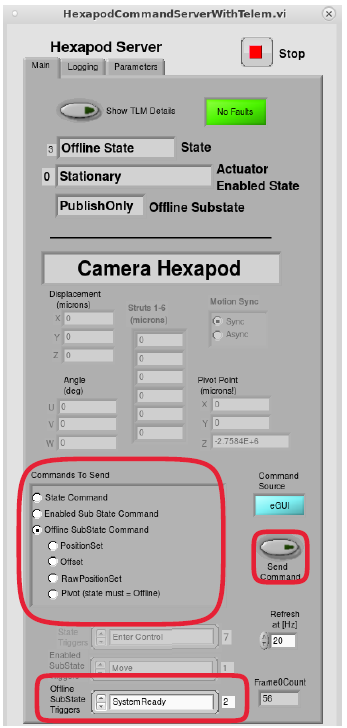
\includegraphics[width=1.79167in]{jira_imgs/1024.png}

}
\hdashrule[0.5ex]{\textwidth}{1pt}{3mm}
  Expected Result \\
{\footnotesize
The system transitions from the OfflineState/PublishOnly substate to the
OfflineState/AvailableState substate.\\[2\baselineskip]

}
\hdashrule[0.5ex]{\textwidth}{1pt}{3mm}
  Actual Result \\
{\footnotesize
We transited the system to the OfflineState/AvailableState substate.

}
\begin{tabular}{p{2cm}p{14cm}}
\toprule
Step 4 & Step Execution Status: \textbf{ Initial Pass } \\ \hline
\end{tabular}
 Description \\
{\footnotesize
\textbf{SWITCHING TO DDS MODE}\\
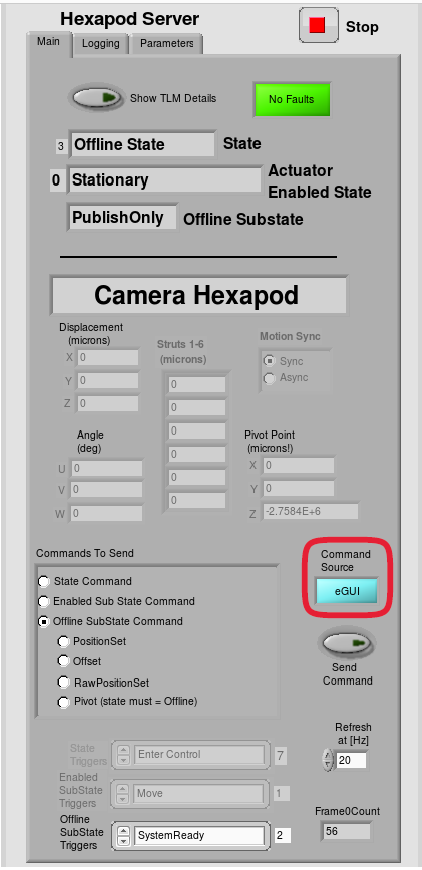
\includegraphics[width=1.68750in]{jira_imgs/1025.png}If the Command
Source does not show DDS, go to the Parameters tab, select DDS under the
Command Source and click the Set Cmd Source button.\\
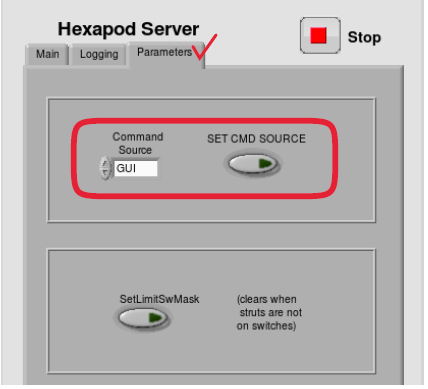
\includegraphics[width=2.34375in]{jira_imgs/1026.png}\textbf{Note:~If
the GUI is used after being set to DDS mode, the system will switch back
the Command Source to GUI and ignore any DDS commands. The Command
Source must show DDS in order to receive DDS commands.}

}
\hdashrule[0.5ex]{\textwidth}{1pt}{3mm}
  Expected Result \\
{\footnotesize
The system is capable of receiving/responding to DDS commands.

}
\hdashrule[0.5ex]{\textwidth}{1pt}{3mm}
  Actual Result \\
{\footnotesize
We can do the DDS control.

}
\begin{tabular}{p{2cm}p{14cm}}
\toprule
Step 5 & Step Execution Status: \textbf{ Initial Pass } \\ \hline
\end{tabular}
 Description \\
{\footnotesize
\textbf{OFFLINESTATE -\textgreater{} STANDBYSTATE}\\
The system receives an enterControl State Transition command through
DDS.

}
\hdashrule[0.5ex]{\textwidth}{1pt}{3mm}
  Expected Result \\
{\footnotesize
The system transitions into the StandbyState and is capable of
receiving/responding to DDS commands.

}
\hdashrule[0.5ex]{\textwidth}{1pt}{3mm}
  Actual Result \\
{\footnotesize
We transited the system to the Standby state.

}
\begin{tabular}{p{2cm}p{14cm}}
\toprule
Step 6 & Step Execution Status: \textbf{ Initial Pass } \\ \hline
\end{tabular}
 Description \\
{\footnotesize
\textbf{STANDBYSTATE -\textgreater{} DISABLEDSTATE}\\
From the StandbyState, send a start command through the DDS.

}
\hdashrule[0.5ex]{\textwidth}{1pt}{3mm}
  Expected Result \\
{\footnotesize
The system transitions into DisabledState after receiving/responding to
DDS command and the wrapper in the PXI real time controller looks for
the configuration file.\\[2\baselineskip]If the configuration file is
invalid or out of range, the system will transition into a Fault State

}
\hdashrule[0.5ex]{\textwidth}{1pt}{3mm}
  Actual Result \\
{\footnotesize
We transited the system to the Disabled state.

}
\begin{tabular}{p{2cm}p{14cm}}
\toprule
Step 7 & Step Execution Status: \textbf{ Initial Pass } \\ \hline
\end{tabular}
 Description \\
{\footnotesize
\textbf{DISABLEDSTATE -\textgreater{} ENABLEDSTATE}\\
From the DisabledState, send an enable state command through the DDS.\\
\textbf{}

}
\hdashrule[0.5ex]{\textwidth}{1pt}{3mm}
  Expected Result \\
{\footnotesize
The system transitions into the EnabledState/Stationary substate, the
motor drives are enabled, motor brakes are released and the system is
capable of receiving/responding to DDS commands.\\[2\baselineskip]

}
\hdashrule[0.5ex]{\textwidth}{1pt}{3mm}
  Actual Result \\
{\footnotesize
We transited the system to the Enabled state.

}
\begin{tabular}{p{2cm}p{14cm}}
\toprule
Step 8 & Step Execution Status: \textbf{ Initial Pass } \\ \hline
\end{tabular}
 Description \\
{\footnotesize
\textbf{FAULTSTATE}\\
If a Fault occurs in any of the other states, the system will
automatically transition to the Fault State. While in the Fault state,
send a clearError command through the DDS.\\
Note: If the fault that occurs goes through the interlock system, reset
the safety relay switch and send a clearError command.

}
\hdashrule[0.5ex]{\textwidth}{1pt}{3mm}
  Expected Result \\
{\footnotesize
The system transitions back to the OfflineState/PublishOnly substate and
is not capable of receiving/responding to DDS commands. (Go back to Step
3)

}
\hdashrule[0.5ex]{\textwidth}{1pt}{3mm}
  Actual Result \\
{\footnotesize
Cleared error and transitioned back to OfflineState/Available

}
\begin{tabular}{p{2cm}p{14cm}}
\toprule
Step 9 & Step Execution Status: \textbf{ Initial Pass } \\ \hline
\end{tabular}
 Description \\
{\footnotesize
\textbf{{MOVE TEST}}\\
\textbf{Section 3.1.2 of the attached Software Acceptance Test
Procedure\\
Test Sequence \#1 - Synchronous PositionSet and Move Commands}\\
In enabled/stationary state, send a positionSet command of (0um, 0um,
200um, 0 deg, 0 deg, 0 deg, s).

}
\hdashrule[0.5ex]{\textwidth}{1pt}{3mm}
  Expected Result \\
{\footnotesize
The hexapod does not move.

}
\hdashrule[0.5ex]{\textwidth}{1pt}{3mm}
  Actual Result \\
{\footnotesize
Did not move.

}
\begin{tabular}{p{2cm}p{14cm}}
\toprule
Step 10 & Step Execution Status: \textbf{ Initial Pass } \\ \hline
\end{tabular}
 Description \\
{\footnotesize
With the synchronous button enabled and in enabled/stationary state,
send a positionSet command of (2000um, -3500um, 200um, 0.01deg, -.05deg,
0.002deg).

}
\hdashrule[0.5ex]{\textwidth}{1pt}{3mm}
  Expected Result \\
{\footnotesize
The hexapod does not move

}
\hdashrule[0.5ex]{\textwidth}{1pt}{3mm}
  Actual Result \\
{\footnotesize
Did not move.

}
\begin{tabular}{p{2cm}p{14cm}}
\toprule
Step 11 & Step Execution Status: \textbf{ Initial Pass } \\ \hline
\end{tabular}
 Description \\
{\footnotesize
Send a move command.

}
\hdashrule[0.5ex]{\textwidth}{1pt}{3mm}
  Expected Result \\
{\footnotesize
\begin{itemize}
\tightlist
\item
  The hexapod moves to (2000um, -3500um, 200um, 0.01deg, -.05deg,
  0.002deg)
\item
  The actuators complete the move at nearly the same time.
\end{itemize}

}
\hdashrule[0.5ex]{\textwidth}{1pt}{3mm}
  Actual Result \\
{\footnotesize
Moved to 1999,-3500,200,0.01,0.05,0.002)

}
\begin{tabular}{p{2cm}p{14cm}}
\toprule
Step 12 & Step Execution Status: \textbf{ Pass w/ Deviation } \\ \hline
\end{tabular}
 Description \\
{\footnotesize
Record the corresponding DDS events that were generated.

}
\hdashrule[0.5ex]{\textwidth}{1pt}{3mm}
  Expected Result \\
{\footnotesize
\begin{itemize}
\tightlist
\item
  The controllerState.enabledSubstate goes to MOVING\_POINT\_TO\_POINT
  when the move begins and STATIONARY when the move ends.
\item
  An inPosition event is generated when the move is complete
\end{itemize}

}
\hdashrule[0.5ex]{\textwidth}{1pt}{3mm}
  Actual Result \\
{\footnotesize
Deviation: Russell will need to modify the XML as the vendor's version
has no Boolean field for inPosition unlike for the Camera Rotator.

}
\hdashrule[0.5ex]{\textwidth}{1pt}{3mm}
  Issues found executing this step:  \\
{\footnotesize
\begin{itemize}
\item \href{https://jira.lsstcorp.org/browse/DM-21699}{DM-21699}~~Clean up XML for (MT) Rotator and Hexapod

\end{itemize}
}
\begin{tabular}{p{2cm}p{14cm}}
\toprule
Step 13 & Step Execution Status: \textbf{ Initial Pass } \\ \hline
\end{tabular}
 Description \\
{\footnotesize
\textbf{Section 3.1.2 of the attached Software Acceptance Test
Procedure\\
Test Sequence \#5 - Stop Commands}\\
In the enabled/stationary state, send a position set command of (0um,
0um, 5000um, 0deg, 0deg, 0deg)

}
\hdashrule[0.5ex]{\textwidth}{1pt}{3mm}
  Expected Result \\
{\footnotesize
The hexapod doesn't move.

}
\hdashrule[0.5ex]{\textwidth}{1pt}{3mm}
  Actual Result \\
{\footnotesize
Does not move

}
\begin{tabular}{p{2cm}p{14cm}}
\toprule
Step 14 & Step Execution Status: \textbf{ Initial Pass } \\ \hline
\end{tabular}
 Description \\
{\footnotesize
Send move command.

}
\hdashrule[0.5ex]{\textwidth}{1pt}{3mm}
  Expected Result \\
{\footnotesize
The hexapod begins to move.

}
\hdashrule[0.5ex]{\textwidth}{1pt}{3mm}
  Actual Result \\
{\footnotesize
Begins to move.

}
\begin{tabular}{p{2cm}p{14cm}}
\toprule
Step 15 & Step Execution Status: \textbf{ Initial Pass } \\ \hline
\end{tabular}
 Description \\
{\footnotesize
Before the hexapod completes its movement, send a stop command.

}
\hdashrule[0.5ex]{\textwidth}{1pt}{3mm}
  Expected Result \\
{\footnotesize
\begin{itemize}
\tightlist
\item
  The hexapod stops before reaching the previously commanded position
\end{itemize}

}
\hdashrule[0.5ex]{\textwidth}{1pt}{3mm}
  Actual Result \\
{\footnotesize
Hexapod stopped

}
\begin{tabular}{p{2cm}p{14cm}}
\toprule
Step 16 & Step Execution Status: \textbf{ Initial Pass } \\ \hline
\end{tabular}
 Description \\
{\footnotesize
Record the corresponding DDS events that were generated.

}
\hdashrule[0.5ex]{\textwidth}{1pt}{3mm}
  Expected Result \\
{\footnotesize
\begin{itemize}
\tightlist
\item
  The controllerState.enabledSubstate goes to CONTROLLED\_STOPPING when
  the stop is requested, then STATIONARY when the hexapod has halted.
\item
  No inPosition event is generated.
\end{itemize}

}
\hdashrule[0.5ex]{\textwidth}{1pt}{3mm}
  Actual Result \\
{\footnotesize
It works.

}
\begin{tabular}{p{2cm}p{14cm}}
\toprule
Step 17 & Step Execution Status: \textbf{ Initial Pass } \\ \hline
\end{tabular}
 Description \\
{\footnotesize
\textbf{Section 3.1.2 of the attached Software Acceptance Test
Procedure\\
Test Sequence \#9 - positionSet and moveLUT}\\
In enabled/stationary state, send a positionSet command of (0um, 0um,
200um, 0deg, 0deg, 0deg)

}
\hdashrule[0.5ex]{\textwidth}{1pt}{3mm}
  Expected Result \\
{\footnotesize
The hexapod doesn't move.

}
\hdashrule[0.5ex]{\textwidth}{1pt}{3mm}
  Actual Result \\
{\footnotesize
Does not move

}
\begin{tabular}{p{2cm}p{14cm}}
\toprule
Step 18 & Step Execution Status: \textbf{ Initial Pass } \\ \hline
\end{tabular}
 Description \\
{\footnotesize
In enabled/stationary state, send a positionSet command of (0um, 0um,
800um, 0deg, 0deg, 0deg)

}
\hdashrule[0.5ex]{\textwidth}{1pt}{3mm}
  Expected Result \\
{\footnotesize
The hexapod doesn't move.

}
\hdashrule[0.5ex]{\textwidth}{1pt}{3mm}
  Actual Result \\
{\footnotesize
Does not move

}
\begin{tabular}{p{2cm}p{14cm}}
\toprule
Step 19 & Step Execution Status: \textbf{ Initial Pass } \\ \hline
\end{tabular}
 Description \\
{\footnotesize
Send a moveLUT (180deg, 60deg, and 10deg) command

}
\hdashrule[0.5ex]{\textwidth}{1pt}{3mm}
  Expected Result \\
{\footnotesize
The hexapod moves to a different position than (0um, 0um, 800um, 0deg,
0deg, 0deg) and the actuators complete the move at nearly the same time.

}
\hdashrule[0.5ex]{\textwidth}{1pt}{3mm}
  Actual Result \\
{\footnotesize
Hexapod moves to a different position(1699,199,920,0.03,-0.02,0.016)
(0,0,2970,0,0,0)

}
\begin{tabular}{p{2cm}p{14cm}}
\toprule
Step 20 & Step Execution Status: \textbf{ Initial Pass } \\ \hline
\end{tabular}
 Description \\
{\footnotesize
{\textbf{OFFSET TEST}}\\
\textbf{Section 3.1.2 of the attached Software Acceptance Test
Procedure\\
Test Sequence \#4 - Synchronous Offset and Move Commands}\\
In enabled/stationary state, send a positionSet command of (500um,
800um, 200um, 0deg, 0deg, 0deg)

}
\hdashrule[0.5ex]{\textwidth}{1pt}{3mm}
  Test Data \\
 {\footnotesize


}
\hdashrule[0.5ex]{\textwidth}{1pt}{3mm}
  Expected Result \\
{\footnotesize
The hexapod doesn't move.

}
\hdashrule[0.5ex]{\textwidth}{1pt}{3mm}
  Actual Result \\
{\footnotesize
Did not move.

}
\begin{tabular}{p{2cm}p{14cm}}
\toprule
Step 21 & Step Execution Status: \textbf{ Initial Pass } \\ \hline
\end{tabular}
 Description \\
{\footnotesize
In enabled/stationary state, send an offset command of (0um, 0um,
2000um, 0deg, 0deg, 0deg).

}
\hdashrule[0.5ex]{\textwidth}{1pt}{3mm}
  Expected Result \\
{\footnotesize
The hexapod doesn't move.

}
\hdashrule[0.5ex]{\textwidth}{1pt}{3mm}
  Actual Result \\
{\footnotesize

}
\begin{tabular}{p{2cm}p{14cm}}
\toprule
Step 22 & Step Execution Status: \textbf{ Initial Pass } \\ \hline
\end{tabular}
 Description \\
{\footnotesize
Send a move command.~

}
\hdashrule[0.5ex]{\textwidth}{1pt}{3mm}
  Expected Result \\
{\footnotesize
\begin{itemize}
\tightlist
\item
  The hexapod moves only 2000um in Z from the previous position
\item
  The actuators complete the move at nearly the same time.
\end{itemize}

}
\hdashrule[0.5ex]{\textwidth}{1pt}{3mm}
  Actual Result \\
{\footnotesize
Works.

}
\begin{tabular}{p{2cm}p{14cm}}
\toprule
Step 23 & Step Execution Status: \textbf{ Pass w/ Deviation } \\ \hline
\end{tabular}
 Description \\
{\footnotesize
Record the corresponding DDS events that were generated.

}
\hdashrule[0.5ex]{\textwidth}{1pt}{3mm}
  Expected Result \\
{\footnotesize
\begin{itemize}
\tightlist
\item
  The controllerState.enabledSubstate goes to MOVING\_POINT\_TO\_POINT
  when the move begins and STATIONARY when the move ends
\item
  The inPosition event is True when the move finishes
\item
  The inPosition event is False when the enabledSubstate goes back to
  STATIONARY.
\end{itemize}

}
\hdashrule[0.5ex]{\textwidth}{1pt}{3mm}
  Actual Result \\
{\footnotesize
Deviation: Russell will need to modify the XML as the vendor's version
has no Boolean field for inPosition unlike for the Camera Rotator.

}
\hdashrule[0.5ex]{\textwidth}{1pt}{3mm}
  Issues found executing this step:  \\
{\footnotesize
\begin{itemize}
\item \href{https://jira.lsstcorp.org/browse/DM-21699}{DM-21699}~~Clean up XML for (MT) Rotator and Hexapod

\end{itemize}
}
\begin{tabular}{p{2cm}p{14cm}}
\toprule
Step 24 & Step Execution Status: \textbf{ Initial Pass } \\ \hline
\end{tabular}
 Description \\
{\footnotesize
\textbf{Section 3.1.2 of the attached Software Acceptance Test
Procedure\\
Test Sequence \#2 -Pivot, PositionSet and Move Commands}\\
In enabled/stationary state, send a positionSet command of (2000um,
-3500um, 200um, 0.01deg, -0.05deg, 0.002deg)

}
\hdashrule[0.5ex]{\textwidth}{1pt}{3mm}
  Test Data \\
 {\footnotesize
\textbf{Deviation:} Determine where the original pivot point is before
sending a pivot command of (0, 0, 0)

}
\hdashrule[0.5ex]{\textwidth}{1pt}{3mm}
  Expected Result \\
{\footnotesize
The hexapod doesn't move.

}
\hdashrule[0.5ex]{\textwidth}{1pt}{3mm}
  Actual Result \\
{\footnotesize
Original pivot is 0, 0, -2.7584E+6

}
\begin{tabular}{p{2cm}p{14cm}}
\toprule
Step 25 & Step Execution Status: \textbf{ Initial Pass } \\ \hline
\end{tabular}
 Description \\
{\footnotesize
In the enabled/stationary state, send a pivot command of (0,0,0).

}
\hdashrule[0.5ex]{\textwidth}{1pt}{3mm}
  Expected Result \\
{\footnotesize
The actuator positions do not change but the hexapod position changes.

}
\hdashrule[0.5ex]{\textwidth}{1pt}{3mm}
  Actual Result \\
{\footnotesize
Position data became -408, -3952, 199, 0.0100 -0.05 0.002

}
\begin{tabular}{p{2cm}p{14cm}}
\toprule
Step 26 & Step Execution Status: \textbf{ Initial Pass } \\ \hline
\end{tabular}
 Description \\
{\footnotesize
In the enabled/stationary state, send a positionSet command of (2000um,
-3500um, 200um, 0.01deg, -0.05deg, 0.002deg)

}
\hdashrule[0.5ex]{\textwidth}{1pt}{3mm}
  Test Data \\
 {\footnotesize
Deviation: Record any offset commands necessary to test before sending
the move command.\\
\textbf{{Note: Need input from Te-Wei on whether there are certain
offset commands to issue before sending the move command.}}

}
\hdashrule[0.5ex]{\textwidth}{1pt}{3mm}
  Expected Result \\
{\footnotesize
The hexapod doesn't move.

}
\hdashrule[0.5ex]{\textwidth}{1pt}{3mm}
  Actual Result \\
{\footnotesize
Does not move

}
\begin{tabular}{p{2cm}p{14cm}}
\toprule
Step 27 & Step Execution Status: \textbf{ Initial Pass } \\ \hline
\end{tabular}
 Description \\
{\footnotesize
Send a move command.

}
\hdashrule[0.5ex]{\textwidth}{1pt}{3mm}
  Expected Result \\
{\footnotesize
Confirm the hexapod moves to the commanded position and the actuators
change position to account for the new pivot point.

}
\hdashrule[0.5ex]{\textwidth}{1pt}{3mm}
  Actual Result \\
{\footnotesize
Moves to 2000, -3500, 200, 0.01, -0.05 0.002

}
\begin{tabular}{p{2cm}p{14cm}}
\toprule
Step 28 & Step Execution Status: \textbf{ Initial Pass } \\ \hline
\end{tabular}
 Description \\
{\footnotesize
\textbf{{CONFIGURE LIMITS TEST}}\\
\textbf{Section 3.1.2 of the attached Software Acceptance Test
Procedure\\
Test Sequence \#6 - configureLimits Command}\\
In enabled/stationary state, send a configureLimits command of (12000um,
-1000um, 1000um, 0.1, -0.1, 0.05)

}
\hdashrule[0.5ex]{\textwidth}{1pt}{3mm}
  Expected Result \\
{\footnotesize
The command is rejected for being outside acceptable limits.

}
\hdashrule[0.5ex]{\textwidth}{1pt}{3mm}
  Actual Result \\
{\footnotesize
Command rejected for x being outside limits

}
\begin{tabular}{p{2cm}p{14cm}}
\toprule
Step 29 & Step Execution Status: \textbf{ Initial Pass } \\ \hline
\end{tabular}
 Description \\
{\footnotesize
In enabled/stationary state, send a configureLimits command of (1000um,
-1000um, 1000um, 0.1, -0.1, 0.05)

}
\hdashrule[0.5ex]{\textwidth}{1pt}{3mm}
  Expected Result \\
{\footnotesize
The command is accepted.

}
\hdashrule[0.5ex]{\textwidth}{1pt}{3mm}
  Actual Result \\
{\footnotesize
Command Accepted

}
\begin{tabular}{p{2cm}p{14cm}}
\toprule
Step 30 & Step Execution Status: \textbf{ Fail } \\ \hline
\end{tabular}
 Description \\
{\footnotesize
In enabled/stationary state, send a positionSet command of (1200um, 0um,
200um, 0deg, 0deg, 0deg)

}
\hdashrule[0.5ex]{\textwidth}{1pt}{3mm}
  Expected Result \\
{\footnotesize
The command is rejected for being outside of range limits

}
\hdashrule[0.5ex]{\textwidth}{1pt}{3mm}
  Actual Result \\
{\footnotesize
Command is accepted. Jira ticket filed~

}
\hdashrule[0.5ex]{\textwidth}{1pt}{3mm}
  Issues found executing this step:  \\
{\footnotesize
\begin{itemize}
\item \href{https://jira.lsstcorp.org/browse/DM-23092}{DM-23092}~~Check position limits for Hexapod move and offset commands

\end{itemize}
}
\begin{tabular}{p{2cm}p{14cm}}
\toprule
Step 31 & Step Execution Status: \textbf{ Fail } \\ \hline
\end{tabular}
 Description \\
{\footnotesize
In enabled/stationary state, send a positionSet command of (990um,
990um, 200um, 0deg, 0deg, 0deg)

}
\hdashrule[0.5ex]{\textwidth}{1pt}{3mm}
  Expected Result \\
{\footnotesize
The command is rejected for being outside of range limits.

}
\hdashrule[0.5ex]{\textwidth}{1pt}{3mm}
  Actual Result \\
{\footnotesize
Command is accepted.

}
\hdashrule[0.5ex]{\textwidth}{1pt}{3mm}
  Issues found executing this step:  \\
{\footnotesize
\begin{itemize}
\item \href{https://jira.lsstcorp.org/browse/DM-23092}{DM-23092}~~Check position limits for Hexapod move and offset commands

\end{itemize}
}
\begin{tabular}{p{2cm}p{14cm}}
\toprule
Step 32 & Step Execution Status: \textbf{ Initial Pass } \\ \hline
\end{tabular}
 Description \\
{\footnotesize
In enabled/stationary state, send a positionSet command of (500um,
500um, 200um, 0deg, 0.1 deg, 0.01deg)

}
\hdashrule[0.5ex]{\textwidth}{1pt}{3mm}
  Expected Result \\
{\footnotesize
The command is accepted.

}
\hdashrule[0.5ex]{\textwidth}{1pt}{3mm}
  Actual Result \\
{\footnotesize
Command accepted.

}
\begin{tabular}{p{2cm}p{14cm}}
\toprule
Step 33 & Step Execution Status: \textbf{ Initial Pass } \\ \hline
\end{tabular}
 Description \\
{\footnotesize
Send a move command.

}
\hdashrule[0.5ex]{\textwidth}{1pt}{3mm}
  Expected Result \\
{\footnotesize
The previously accepted command is executed.

}
\hdashrule[0.5ex]{\textwidth}{1pt}{3mm}
  Actual Result \\
{\footnotesize
Move completed to correct position

}
\begin{tabular}{p{2cm}p{14cm}}
\toprule
Step 34 & Step Execution Status: \textbf{ In Progress } \\ \hline
\end{tabular}
 Description \\
{\footnotesize
Record the DDS events that were generated.

}
\hdashrule[0.5ex]{\textwidth}{1pt}{3mm}
  Expected Result \\
{\footnotesize
The change is reflected in the settingsApplied event and the EUI.

}
\hdashrule[0.5ex]{\textwidth}{1pt}{3mm}
  Actual Result \\
{\footnotesize
Change reflected in EUI, still checking EFD.

}
\begin{tabular}{p{2cm}p{14cm}}
\toprule
Step 35 & Step Execution Status: \textbf{ Initial Pass } \\ \hline
\end{tabular}
 Description \\
{\footnotesize
{\textbf{CONFIGURE ACCELERATION TEST}}\\
\textbf{Section 3.1.2 of the attached Software Acceptance Test
Procedure\\
Test Sequence \#7 - configureAcceleration Command}\\
In enabled/stationary state, at a position of (0, 0, 0, 0, 0, 0) with
the velocity and acceleration values set to their nominal values, send a
positionSet command of (0um, 0um, 4900um, 0 deg, 0 deg, 0 deg, s).

}
\hdashrule[0.5ex]{\textwidth}{1pt}{3mm}
  Expected Result \\
{\footnotesize
The hexapod doesn't move.

}
\hdashrule[0.5ex]{\textwidth}{1pt}{3mm}
  Actual Result \\
{\footnotesize
The Hexapod does not move

}
\begin{tabular}{p{2cm}p{14cm}}
\toprule
Step 36 & Step Execution Status: \textbf{ Initial Pass } \\ \hline
\end{tabular}
 Description \\
{\footnotesize
Send a move command.

}
\hdashrule[0.5ex]{\textwidth}{1pt}{3mm}
  Expected Result \\
{\footnotesize
The move takes approximately 9 seconds to complete.

}
\hdashrule[0.5ex]{\textwidth}{1pt}{3mm}
  Actual Result \\
{\footnotesize
Hexapod movement took approximately 9 seconds.~

}
\begin{tabular}{p{2cm}p{14cm}}
\toprule
Step 37 & Step Execution Status: \textbf{ Initial Pass } \\ \hline
\end{tabular}
 Description \\
{\footnotesize
Send a configureAcceleration command of 1000.

}
\hdashrule[0.5ex]{\textwidth}{1pt}{3mm}
  Expected Result \\
{\footnotesize
~Confirm command is rejected for being outside of acceptable limits.

}
\hdashrule[0.5ex]{\textwidth}{1pt}{3mm}
  Actual Result \\
{\footnotesize
Command rejected

}
\begin{tabular}{p{2cm}p{14cm}}
\toprule
Step 38 & Step Execution Status: \textbf{ Initial Pass } \\ \hline
\end{tabular}
 Description \\
{\footnotesize
Send a configureAcceleration command of 100.

}
\hdashrule[0.5ex]{\textwidth}{1pt}{3mm}
  Expected Result \\
{\footnotesize
The command is accepted.~

}
\hdashrule[0.5ex]{\textwidth}{1pt}{3mm}
  Actual Result \\
{\footnotesize
Command accepted

}
\begin{tabular}{p{2cm}p{14cm}}
\toprule
Step 39 & Step Execution Status: \textbf{ Initial Pass } \\ \hline
\end{tabular}
 Description \\
{\footnotesize
In enabled/stationary state, send a postionSet command of (0um, 0um,
0um, 0 deg, 0 deg, 0 deg, s).

}
\hdashrule[0.5ex]{\textwidth}{1pt}{3mm}
  Expected Result \\
{\footnotesize
The hexapod doesn't move.

}
\hdashrule[0.5ex]{\textwidth}{1pt}{3mm}
  Actual Result \\
{\footnotesize
Hexapod does not move

}
\begin{tabular}{p{2cm}p{14cm}}
\toprule
Step 40 & Step Execution Status: \textbf{ Initial Pass } \\ \hline
\end{tabular}
 Description \\
{\footnotesize
Send a move command.~

}
\hdashrule[0.5ex]{\textwidth}{1pt}{3mm}
  Expected Result \\
{\footnotesize
It takes approximately 13 seconds to complete the commanded move with
the reduced acceleration value.

}
\hdashrule[0.5ex]{\textwidth}{1pt}{3mm}
  Actual Result \\
{\footnotesize
Hexapod moved in approximately~ 13 seconds.

}
\begin{tabular}{p{2cm}p{14cm}}
\toprule
Step 41 & Step Execution Status: \textbf{ Initial Pass } \\ \hline
\end{tabular}
 Description \\
{\footnotesize
Send a configureAcceleration command of 500 to return the acceleration
limit to its nominal value.

}
\hdashrule[0.5ex]{\textwidth}{1pt}{3mm}
  Expected Result \\
{\footnotesize
The command is accepted.

}
\hdashrule[0.5ex]{\textwidth}{1pt}{3mm}
  Actual Result \\
{\footnotesize
Command accepted

}
\begin{tabular}{p{2cm}p{14cm}}
\toprule
Step 42 & Step Execution Status: \textbf{ In Progress } \\ \hline
\end{tabular}
 Description \\
{\footnotesize
Record the corresponding DDS events that were generated.

}
\hdashrule[0.5ex]{\textwidth}{1pt}{3mm}
  Expected Result \\
{\footnotesize
The change is reflected in the settingsApplied event and the EUI.

}
\hdashrule[0.5ex]{\textwidth}{1pt}{3mm}
  Actual Result \\
{\footnotesize
Changes were evident in EUI, still need to find EFD.

}
\begin{tabular}{p{2cm}p{14cm}}
\toprule
Step 43 & Step Execution Status: \textbf{ Initial Pass } \\ \hline
\end{tabular}
 Description \\
{\footnotesize
\textbf{{CONFIGURE VELOCITY TEST}}\\
\textbf{Section 3.1.2 of the attached Software Acceptance Test
Procedure\\
Test Sequence \#8 - configureVelocity Command}\\
In enabled/stationary state, at a position of (0, 0, 0, 0, 0, 0), send a
configureVelocity command of (10000, .01, 100, .01).

}
\hdashrule[0.5ex]{\textwidth}{1pt}{3mm}
  Expected Result \\
{\footnotesize
This command is rejected for being outside of acceptable limits.

}
\hdashrule[0.5ex]{\textwidth}{1pt}{3mm}
  Actual Result \\
{\footnotesize
Command rejected

}
\begin{tabular}{p{2cm}p{14cm}}
\toprule
Step 44 & Step Execution Status: \textbf{ Initial Pass } \\ \hline
\end{tabular}
 Description \\
{\footnotesize
In enabled/stationary state, send a configureVelocity command of (100,
.01, 200, .01).~

}
\hdashrule[0.5ex]{\textwidth}{1pt}{3mm}
  Expected Result \\
{\footnotesize
This command is accepted.

}
\hdashrule[0.5ex]{\textwidth}{1pt}{3mm}
  Actual Result \\
{\footnotesize
Command accepted

}
\begin{tabular}{p{2cm}p{14cm}}
\toprule
Step 45 & Step Execution Status: \textbf{ Initial Pass } \\ \hline
\end{tabular}
 Description \\
{\footnotesize
In enabled/stationary state, send a positionSet command of (0, 0um,
2000um, 0 deg, 0 deg, 0 deg, s).

}
\hdashrule[0.5ex]{\textwidth}{1pt}{3mm}
  Expected Result \\
{\footnotesize
The command is accepted

}
\hdashrule[0.5ex]{\textwidth}{1pt}{3mm}
  Actual Result \\
{\footnotesize
Command accepted

}
\begin{tabular}{p{2cm}p{14cm}}
\toprule
Step 46 & Step Execution Status: \textbf{ Initial Pass } \\ \hline
\end{tabular}
 Description \\
{\footnotesize
Send a move command.~

}
\hdashrule[0.5ex]{\textwidth}{1pt}{3mm}
  Expected Result \\
{\footnotesize
It takes approximately 20 seconds to complete the commanded move.

}
\hdashrule[0.5ex]{\textwidth}{1pt}{3mm}
  Actual Result \\
{\footnotesize
Approximately 20 seconds taken to move

}
\begin{tabular}{p{2cm}p{14cm}}
\toprule
Step 47 & Step Execution Status: \textbf{ Initial Pass } \\ \hline
\end{tabular}
 Description \\
{\footnotesize
In enabled/stationary state, send a configureVelocity command of (100,
.01, 100, .01).~

}
\hdashrule[0.5ex]{\textwidth}{1pt}{3mm}
  Expected Result \\
{\footnotesize
This command is accepted.

}
\hdashrule[0.5ex]{\textwidth}{1pt}{3mm}
  Actual Result \\
{\footnotesize
Accepted

}
\begin{tabular}{p{2cm}p{14cm}}
\toprule
Step 48 & Step Execution Status: \textbf{ Initial Pass } \\ \hline
\end{tabular}
 Description \\
{\footnotesize
In enabled/stationary state, send an offset command of (0, 0um, 2000um,
0 deg, 0 deg, 0 deg).

}
\hdashrule[0.5ex]{\textwidth}{1pt}{3mm}
  Expected Result \\
{\footnotesize
This command is accepted

}
\hdashrule[0.5ex]{\textwidth}{1pt}{3mm}
  Actual Result \\
{\footnotesize
Command accepted

}
\begin{tabular}{p{2cm}p{14cm}}
\toprule
Step 49 & Step Execution Status: \textbf{ Initial Pass } \\ \hline
\end{tabular}
 Description \\
{\footnotesize
Send a move command.~

}
\hdashrule[0.5ex]{\textwidth}{1pt}{3mm}
  Expected Result \\
{\footnotesize
It takes approximately 40 seconds to complete the commanded move.

}
\hdashrule[0.5ex]{\textwidth}{1pt}{3mm}
  Actual Result \\
{\footnotesize
Move completed in 40 seconds

}
\begin{tabular}{p{2cm}p{14cm}}
\toprule
Step 50 & Step Execution Status: \textbf{ In Progress } \\ \hline
\end{tabular}
 Description \\
{\footnotesize
Record the corresponding DDS events that were generated:

}
\hdashrule[0.5ex]{\textwidth}{1pt}{3mm}
  Expected Result \\
{\footnotesize
The change is reflected in the settingsApplied event and the EUI.

}
\hdashrule[0.5ex]{\textwidth}{1pt}{3mm}
  Actual Result \\
{\footnotesize
Changes reflected in EUI, still determining EFD

}
\begin{tabular}{p{2cm}p{14cm}}
\toprule
Step 51 & Step Execution Status: \textbf{ Initial Pass } \\ \hline
\end{tabular}
 Description \\
{\footnotesize
\textbf{Section 3.3.2 of the attached Software Acceptance Test Procedure
Hexapod Action on State Commands}\\
In the Offline/PublishOnly state, send all commands

}
\hdashrule[0.5ex]{\textwidth}{1pt}{3mm}
  Expected Result \\
{\footnotesize
There is no change and command is rejected.

}
\hdashrule[0.5ex]{\textwidth}{1pt}{3mm}
  Actual Result \\
{\footnotesize

}
\begin{tabular}{p{2cm}p{14cm}}
\toprule
Step 52 & Step Execution Status: \textbf{ Initial Pass } \\ \hline
\end{tabular}
 Description \\
{\footnotesize
In the Offline/Available state, send an enterControl command

}
\hdashrule[0.5ex]{\textwidth}{1pt}{3mm}
  Expected Result \\
{\footnotesize
The system enters the Standby state.

}
\hdashrule[0.5ex]{\textwidth}{1pt}{3mm}
  Actual Result \\
{\footnotesize
System enters standby state

}
\begin{tabular}{p{2cm}p{14cm}}
\toprule
Step 53 & Step Execution Status: \textbf{ Initial Pass } \\ \hline
\end{tabular}
 Description \\
{\footnotesize
In the Standby state, send any command except start or exitControl

}
\hdashrule[0.5ex]{\textwidth}{1pt}{3mm}
  Expected Result \\
{\footnotesize
There is no change and command is rejected.

}
\hdashrule[0.5ex]{\textwidth}{1pt}{3mm}
  Actual Result \\
{\footnotesize
Command rejected

}
\begin{tabular}{p{2cm}p{14cm}}
\toprule
Step 54 & Step Execution Status: \textbf{ Initial Pass } \\ \hline
\end{tabular}
 Description \\
{\footnotesize
In the Standby state, send an exitControl command.

}
\hdashrule[0.5ex]{\textwidth}{1pt}{3mm}
  Expected Result \\
{\footnotesize
The system transitions into the Offline/Available state.

}
\hdashrule[0.5ex]{\textwidth}{1pt}{3mm}
  Actual Result \\
{\footnotesize
Transitions to Offline/Available

}
\begin{tabular}{p{2cm}p{14cm}}
\toprule
Step 55 & Step Execution Status: \textbf{ Initial Pass } \\ \hline
\end{tabular}
 Description \\
{\footnotesize
In the Standby state, send a start command.

}
\hdashrule[0.5ex]{\textwidth}{1pt}{3mm}
  Expected Result \\
{\footnotesize
The system transitions into the Disabled state.

}
\hdashrule[0.5ex]{\textwidth}{1pt}{3mm}
  Actual Result \\
{\footnotesize
Transitions to disabled state

}
\begin{tabular}{p{2cm}p{14cm}}
\toprule
Step 56 & Step Execution Status: \textbf{ Initial Pass } \\ \hline
\end{tabular}
 Description \\
{\footnotesize
In the Disabled state, send any command except for the enabled or
standby command.

}
\hdashrule[0.5ex]{\textwidth}{1pt}{3mm}
  Expected Result \\
{\footnotesize
There is no change and the command is rejected.

}
\hdashrule[0.5ex]{\textwidth}{1pt}{3mm}
  Actual Result \\
{\footnotesize
Command rejected

}
\begin{tabular}{p{2cm}p{14cm}}
\toprule
Step 57 & Step Execution Status: \textbf{ Initial Pass } \\ \hline
\end{tabular}
 Description \\
{\footnotesize
In the Disabled state, send the standby command.

}
\hdashrule[0.5ex]{\textwidth}{1pt}{3mm}
  Expected Result \\
{\footnotesize
The system transitions into the Standby state.

}
\hdashrule[0.5ex]{\textwidth}{1pt}{3mm}
  Actual Result \\
{\footnotesize
Transitions to standby state

}
\begin{tabular}{p{2cm}p{14cm}}
\toprule
Step 58 & Step Execution Status: \textbf{ Initial Pass } \\ \hline
\end{tabular}
 Description \\
{\footnotesize
In the Disabled state, send the enable command.

}
\hdashrule[0.5ex]{\textwidth}{1pt}{3mm}
  Expected Result \\
{\footnotesize
The system transitions into the Enabled/Stationary state.

}
\hdashrule[0.5ex]{\textwidth}{1pt}{3mm}
  Actual Result \\
{\footnotesize
Transitions to enabled state

}
\begin{tabular}{p{2cm}p{14cm}}
\toprule
Step 59 & Step Execution Status: \textbf{ Initial Pass } \\ \hline
\end{tabular}
 Description \\
{\footnotesize
In the Enabled/Stationary state, send either the enterControl command,
exitControl command, start command, clearError command, or enable
command.

}
\hdashrule[0.5ex]{\textwidth}{1pt}{3mm}
  Expected Result \\
{\footnotesize
There is no change and command is rejected.

}
\hdashrule[0.5ex]{\textwidth}{1pt}{3mm}
  Actual Result \\
{\footnotesize
Command rejected

}
\begin{tabular}{p{2cm}p{14cm}}
\toprule
Step 60 & Step Execution Status: \textbf{ Initial Pass } \\ \hline
\end{tabular}
 Description \\
{\footnotesize
In the Enabled/Stationary state, send a disable command.

}
\hdashrule[0.5ex]{\textwidth}{1pt}{3mm}
  Expected Result \\
{\footnotesize
The system transitions into Disabled state.

}
\hdashrule[0.5ex]{\textwidth}{1pt}{3mm}
  Actual Result \\
{\footnotesize
Transitioned to disabled state

}
\begin{tabular}{p{2cm}p{14cm}}
\toprule
Step 61 & Step Execution Status: \textbf{ Initial Pass } \\ \hline
\end{tabular}
 Description \\
{\footnotesize
In the Fault state, send any command except the clearError command.

}
\hdashrule[0.5ex]{\textwidth}{1pt}{3mm}
  Expected Result \\
{\footnotesize
There is no change and command is rejected.

}
\hdashrule[0.5ex]{\textwidth}{1pt}{3mm}
  Actual Result \\
{\footnotesize

}
\begin{tabular}{p{2cm}p{14cm}}
\toprule
Step 62 & Step Execution Status: \textbf{ Initial Pass } \\ \hline
\end{tabular}
 Description \\
{\footnotesize
In the Fault state, send the clearError command.

}
\hdashrule[0.5ex]{\textwidth}{1pt}{3mm}
  Expected Result \\
{\footnotesize
The system transitions into the Offline/PublishOnly state.

}
\hdashrule[0.5ex]{\textwidth}{1pt}{3mm}
  Actual Result \\
{\footnotesize

}
\begin{tabular}{p{2cm}p{14cm}}
\toprule
Step 63 & Step Execution Status: \textbf{ Not Executed } \\ \hline
\end{tabular}
 Description \\
{\footnotesize
\textbf{Section 4 of the attached Software Acceptance Test Procedure}\\
In the Enabled/Stationary state, unplug a motor encoder cable for one of
the actuators.\textbf{}\\

}
\hdashrule[0.5ex]{\textwidth}{1pt}{3mm}
  Expected Result \\
{\footnotesize
A Drive Fault error event is created and the system transitions to Fault
state.

}
\hdashrule[0.5ex]{\textwidth}{1pt}{3mm}
  Actual Result \\
{\footnotesize

}
\begin{tabular}{p{2cm}p{14cm}}
\toprule
Step 64 & Step Execution Status: \textbf{ Not Executed } \\ \hline
\end{tabular}
 Description \\
{\footnotesize
In the Enabled/Stationary state, unplug a linear encoder cable for one
of the actuators.

}
\hdashrule[0.5ex]{\textwidth}{1pt}{3mm}
  Expected Result \\
{\footnotesize
A Drive Fault error event is created and the system transitions to Fault
state.

}
\hdashrule[0.5ex]{\textwidth}{1pt}{3mm}
  Actual Result \\
{\footnotesize

}
\begin{tabular}{p{2cm}p{14cm}}
\toprule
Step 65 & Step Execution Status: \textbf{ Not Executed } \\ \hline
\end{tabular}
 Description \\
{\footnotesize
Unplug a motor power cable from one of the actuators and command a
PositionSet/Move.

}
\hdashrule[0.5ex]{\textwidth}{1pt}{3mm}
  Expected Result \\
{\footnotesize
A Following Error event is created and the system transitions to Fault
state.

}
\hdashrule[0.5ex]{\textwidth}{1pt}{3mm}
  Actual Result \\
{\footnotesize

}
\begin{tabular}{p{2cm}p{14cm}}
\toprule
Step 66 & Step Execution Status: \textbf{ Not Executed } \\ \hline
\end{tabular}
 Description \\
{\footnotesize
Activate an extension limit switch on one of the actuators by removing
the limit switch cover and manually tripping.

}
\hdashrule[0.5ex]{\textwidth}{1pt}{3mm}
  Expected Result \\
{\footnotesize
An Extended Limit Switch error event is created and the system
transitions into Fault state.

}
\hdashrule[0.5ex]{\textwidth}{1pt}{3mm}
  Actual Result \\
{\footnotesize

}
\begin{tabular}{p{2cm}p{14cm}}
\toprule
Step 67 & Step Execution Status: \textbf{ Not Executed } \\ \hline
\end{tabular}
 Description \\
{\footnotesize
Activate a retraction limit switch on one of the actuators by removing
the limit switch cover and manually tripping.

}
\hdashrule[0.5ex]{\textwidth}{1pt}{3mm}
  Expected Result \\
{\footnotesize
A Retracted Limit Switch error event is created and the system
transitions into Fault state.

}
\hdashrule[0.5ex]{\textwidth}{1pt}{3mm}
  Actual Result \\
{\footnotesize

}
\begin{tabular}{p{2cm}p{14cm}}
\toprule
Step 68 & Step Execution Status: \textbf{ Not Executed } \\ \hline
\end{tabular}
 Description \\
{\footnotesize
Unplug the Ethercat cable between the control PC and the first Copley
XE2 drive.

}
\hdashrule[0.5ex]{\textwidth}{1pt}{3mm}
  Expected Result \\
{\footnotesize
An Ethercat Lost event is created and the system transitions to Fault
state.

}
\hdashrule[0.5ex]{\textwidth}{1pt}{3mm}
  Actual Result \\
{\footnotesize

}



\newpage
\appendix
%Make sure lsst-texmf/bin/generateAcronyms.py is in your path
\section{Acronyms used in this document}\label{sec:acronyms}
\addtocounter{table}{-1}
\begin{longtable}{p{0.145\textwidth}p{0.8\textwidth}}\hline
\textbf{Acronym} & \textbf{Description}  \\\hline

EFD & Engineering and Facility Database \\\hline
GUI & Graphical User Interface \\\hline
LSST & Large Synoptic Survey Telescope \\\hline
LUT & Look-Up Table \\\hline
PMCS & Project Management Controls System \\\hline
Source & A single detection of an astrophysical object in an image, the characteristics for which are stored in the Source Catalog of the DRP database. The association of Sources that are non-moving lead to Objects; the association of moving Sources leads to Solar System Objects. (Note that in non-LSST usage "source" is often used for what LSST calls an Object.) \\\hline
\end{longtable}


\end{document}
